\documentclass[ENG]{TFUOC}%IB: CASTELLÀ, CAT: CATALÀ, ENG: ANGLISH

%Other packages
\usepackage{hyperref}
\usepackage{booktabs}
\usepackage{adjustbox}
\usepackage{graphicx}
\usepackage{subcaption}
\usepackage{fancyvrb}
\usepackage{fvextra}
\usepackage{listings}
\usepackage{float}
\usepackage{longtable}
\usepackage{comment} 

%Introduce Work Data
\title{Integrative Analysis of Differential Gene Expression, Transcript Usage, and RNA Secondary Structure in Early- and Late-Onset Colorectal Cancer}
\titcrt{DGE, DTU, and RSS analyses in CRC} %Short title to appear in header
\author{Salomon Elieser Marquez Villalobos}
\date{\today}

\nomPDC{Fernando Pastor Rodriguez and Igor Ruiz de los Mozos Aliaga}
\nomPRA{Diego Garrido Martin}
\titulac{Master in Bioinformatics and Bioestadistics}
\area{M0.207 Omics Data Analysis}
\idioma{English}
\credits{15}
\parcla{CRC, DGE, DTU, 2D RNA structure prediction}

\licenc{ccBy}
%Possible licenses
%ccByNcNd
%ccByNcSa
%ccByNc
%ccByNd
%ccBySa
%ccBy
%GNU
%copyright


%%%%%%%%%%
% Summary in language

%\abstractidioma{
%Maximum 250 words, for the purpose, context of application, methodology, results and conclusions of the work.
%}

% Summary in English.
\abstractenglish{
Colorectal cancer is increasingly diagnosed in individuals younger than 50 years, a trend referred to as early-onset colorectal cancer. This study applied an integrative transcriptomic workflow to characterize molecular differences between early-onset and late-onset colorectal cancer. A total of 86 matched tumor and normal samples were analyzed using a combination of differential gene expression, differential transcript usage, and RNA secondary structure prediction.

Differential gene expression analysis identified a 40-gene signature uniquely deregulated in early-onset colorectal cancer, enriched in immune-related, inflammatory, and cell-matrix adhesion processes. Differential transcript usage analysis revealed substantial differences in transcript-level complexity between cohorts, with late-onset colorectal cancer showing extensive isoform remodeling, whereas early-onset tumors displayed a more restricted pattern of transcript usage. Despite these global differences, six conserved isoform switches were consistently detected in both cohorts, including TPM2, LMNB2, MAP3K20, and the long non-coding RNA HOXB-AS3. RNA secondary structure prediction further characterized significant isoforms, revealing a predominance of stem motifs.

These results indicate that gene-level and isoform-level analyses capture complementary aspects of colorectal cancer transcriptomic variation. The integrative framework presented here provides a methodological basis for future large-scale studies and supports the exploration of RNA structural features as potential biomarkers and therapeutic targets in colorectal cancer.
}

\begin{document}

\estructura

\chapter*{Acknowledgements}

\begin{description}

\item To my wife, Angeles, for her unconditional support and affection, and for introducing me to the world of biology and gene therapy.

\item To my father, Felix and Martina, for their hospitality and care during the writing of this manuscript.

\item To my supervisors. Fernando, thank you for welcoming me into your laboratory and for providing all the resources necessary to complete this project. Igor, thank you for your experience and guidance, for being a facilitator who shared his passion for teaching.

\item To my tutor, Diego, for his observations during the execution of this work.

\end{description}

\tableofcontents

\listoffigures

\listoftables

%-----------------------------------------------------------
\chapter{Introduction}

Colorectal cancer (CRC) is one of the leading causes of cancer-related morbidity and mortality worldwide \cite{vogelsteinCancerGenomeLandscapes2013}. Traditionally regarded as a disease predominantly affecting older individuals, recent years have seen a marked increase in cases diagnosed in patients under 50 years of age \cite{marxIdentificationDifferentiallyExpressed2024}. This trend, referred to as early-onset colorectal cancer (EOCRC), is associated with distinct clinical, molecular, and prognostic characteristics. Compared with late-onset colorectal cancer (LOCRC), EOCRC tumors more frequently exhibit signet ring cell features \cite{willauerClinicalMolecularCharacterization2019}, tend to arise in the distal colon or rectum \cite{burnett-hartmanTreatmentPatternsSurvival2019}, and display distinct mutational landscapes, including a lower prevalence of APC-mutated tumors \cite{xuGermlineProfilingMolecular2020}. Elucidating the molecular mechanisms that differentiate EOCRC from LOCRC is therefore critical for improving early detection strategies and guiding more effective therapeutic approaches. 

\section*{Transcriptome profiling in CRC}

Transcriptome analysis using RNA sequencing (RNA-seq) has become a cornerstone in the molecular investigation of colorectal cancer, enabling the identification of genes that are differentially expressed between pathological conditions and healthy controls. This approach has substantially contributed to the discovery of dysregulated pathways and candidate biomarkers associated with colorectal carcinogenesis. A number of studies have reported genes whose expression appears to be associated with EOCRC, including ALDH1A1 \cite{vermaniExpressionPatternAldh12020}, PEG10 \cite{watsonDifferentialExpressionPEG102020}, and ANPEP \cite{haReducedExpressionAlanyl2023}. Although differences in mutational landscapes between early-onset and late-onset colorectal cancer have been investigated in previous studies \cite{yanOrganoidCulturesEarlyonset2020}, comparative analyses of their transcriptional profiles remain relatively limited and have only gained attention in recent years. 

\section*{Isoform diversity and alternative splicing in CRC}

Gene-level differential expression analyses (DGE) provide only a partial representation of the transcriptomic complexity, as a single gene can give rise to multiple transcript isoforms with distinct regulatory and functional properties. Biologically meaningful alterations may occur at the transcript level without being reflected in changes in total gene expression. In this regard, most existing transcriptomic studies of EOCRC \cite{marxMolecularGeneticsEarlyonset2023} have focused primarily on gene-level expression changes, thereby overlooking post-transcriptional regulatory mechanisms that can contribute significantly to transcriptome complexity. 

Alternative splicing is a central mechanism of post-transcriptional regulation that increases proteomic diversity by generating multiple mRNA isoforms from the same gene. Importantly, alternative splicing is a major driver of functional diversity in colorectal cancer \cite{hallRNASplicingKey2022} and is known to be influenced by age, environmental factors \cite{bhadraAlternativeSplicingAging2020}, and the intestinal microbiome \cite{martinez-montielMicrobialNaturalMetabolites2016}. Aberrant splicing patterns have been widely implicated in the initiation and progression of colorectal cancer and other solid tumors. Despite its biological relevance, isoform-level regulation has not been extensively characterized in EOCRC. 

Differential transcript usage (DTU) analysis allows for the detection of changes in the relative proportions of isoforms between conditions independently of gene-level expression differences, offering isoform-specific resolution. Tools such as \texttt{IsoformSwitchAnalyzeR} \cite{vitting-seerupIsoformSwitchAnalyzeRAnalysisChanges2019} enable the systematic characterization of changes in exon usage, untranslated regions, intron retention, and open reading frames, thereby linking transcript-level variation to potential functional outcomes. Consequently, integrating DGE and DTU analyses can provide a mechanistic framework to interpret how changes in isoform usage may lead to functional divergence beyond expression levels alone in CRC. Addressing this task requires bioinformatics approaches capable of resolving transcript-level variation and integrating it with downstream functional analyses.

\section*{RNA structure as a functional layer of transcriptomic regulation in CRC}

The function of RNA is not determined solely by its nucleotide sequence or expression level, it is also shaped by the conformations it adopts. RNA molecules can adopt a wide range of structures that are essential for their biological roles \cite{caoIdentificationRNAStructures2024}, such as tRNAs, small nucleolar RNAs, ribosomal RNAs and riboswitches, yet the principles governing RNA folding and the functional relevance of many structural elements remain incompletely understood. As a result, studying the dynamics and functional impact of RNA structure has emerged as a central area of investigation in modern molecular biology.

A practical way to explore how RNA molecules may adopt specific conformations is through computational structure prediction, particularly in cases where experimental determination of RNA structure is not feasible. These approaches are generally most reliable for shorter transcripts, while prediction complexity and uncertainty increase substantially with RNA length. A wide range of algorithms has been developed to infer RNA secondary structures using thermodynamic principles \cite{reuterRNAstructureSoftwareRNA2010,lorenzViennaRNAPackage202011}, comparative approaches that exploit sequence covariation \cite{hofackerSecondaryStructurePrediction2002,washietlFastReliablePrediction2005,rivasStatisticalTestConserved2017}, and machine learning and artificial intelligence–based strategies \cite{satoRecentTrendsRNA2023a}. Furthermore, motivated by the success of large language models (LLMs) in proteins and DNA \cite{linBridgingArtificialIntelligence2025}, a number of RNA-focused LLMs have recently been developed \cite{zablockiComprehensiveBenchmarkingLarge2025} being RNA secondary structure prediction one of their most relevant and impactful applications.

Considering the clinical and molecular differences between younger and older patients with CRC, it is of particular interest to investigate whether age-associated changes in isoform usage translate into alterations in RNA structure. Identifying differentially used transcripts between age groups and analyzing their secondary structures could reveal regulatory mechanisms specific to EOCRC or LOCRC patients.

\section{Work objectives}

\subsection{General objective}
The primary goal of this project is to identify genes and transcripts that are differentially regulated in early-onset and late-onset colorectal cancer, and to evaluate whether changes in isoform usage are associated with differences in their RNA secondary structure through computational prediction.

\subsection{Specific objectives}

\begin{itemize}
    \item Identify genes differentially expressed between EOCRC and LOCRC samples and characterize the biological pathways associated with transcriptional changes.
    \item Detect and characterize transcripts exhibiting significant differential usage between EOCRC and LOCRC samples, with emphasis on isoform switching events and alternative splicing.
    \item Evaluate whether age-associated isoform switches in CRC are associated with changes in predicted RNA secondary structure.
\end{itemize}

\section{Focus and method followed}

In this work, we adopted an integrative transcriptomic strategy to investigate molecular differences between early-onset and late-onset colorectal cancer (EOCRC and LOCRC). Building upon a previously conducted gene-level study \cite{marxIdentificationDifferentiallyExpressed2024}, we extend the analysis by incorporating isoform-level regulation and RNA secondary structure prediction, thereby moving beyond expression changes alone to explore post-transcriptional and structural layers of regulation.

Publicly available RNA-seq datasets comprising paired tumor and adjacent normal tissues from EOCRC and LOCRC patients were analyzed to characterize transcriptional regulation at both the gene and isoform levels. Gene-level differential expression analysis (DGE) was performed to establish a baseline view of age-associated transcriptional differences and to identify dysregulated biological pathways. Building on this framework, differential transcript usage (DTU) analyses were conducted to detect changes in isoform proportions, with particular emphasis on alternative splicing and isoform switching events that are not captured by gene-centric approaches.

To investigate the potential functional consequences of age-associated isoform regulation, transcripts exhibiting significant differential usage were further analyzed using computational RNA secondary structure prediction. Predicted structures were assessed both qualitatively and quantitatively to identify structural motifs and features that may differ between age groups, using RNAstructure and the \textit{bpRNA} toolkit. By integrating gene-level expression, isoform-level regulation, and RNA structural analysis, this study aims to provide a multi-layered view of transcriptomic complexity in colorectal cancer and to assess whether age-dependent isoform usage is associated with structural features of potential functional relevance.

\section{Working Plan}
The main milestones for this project are outlined below. Progress was tracked in real time using a dedicated \href{https://github.com/users/sblaizerwize/projects/5/views/4?visibleFields=%5B%22Title%22%2C%22Status%22%2C%22Milestone%22%2C224733603%2C224733604%5D&sortedBy%5Bdirection%5D=asc&sortedBy%5BcolumnId%5D=224733604}{master-bioinformatics GitHub project}, which facilitated version control, documentation of analytical decisions, and reproducibility of results. 

\begin{itemize}
    \item M1 (by October 31): RNA-seq processing pipeline deployed and validated on the UNAV HPC cluster, with gene- and transcript-level quantification completed for EOCRC and LOCRC cohorts.
    \item M2 (by November 30): Differential gene expression and differential transcript usage analyses finalized, including functional and splicing consequence annotation of significant isoform switches.
    \item M3 (by December 15): RNA secondary structure prediction and structural motif analysis of age-associated isoform switches completed.
    \item M4 (by December 31): Final manuscript submitted to advisors.
\end{itemize}

\subsection{Retrospective risk analysis}

Table~\ref{tab:risk_analysis} summarizes the main technical and methodological challenges
encountered during the development of this project and the mitigation
strategies adopted. Detailed progress reports, intermediate analyses, and implementation decisions are available in the \href{https://github.com/sblaizerwize/master-bioinformatics/tree/main/writing/tfm-progress-reports}{master-bioinformatics GitHub repository}, ensuring full reproducibility and transparency of the workflow.

\begin{table}[!h]
\centering
\caption{Retrospective analysis of major challenges to implement the project, their impact, and mitigation strategies adopted.}
\label{tab:risk_analysis}
\renewcommand{\arraystretch}{1.2}
\begin{tabular}{p{3.5cm} p{5.5cm} p{5.5cm}}
\toprule
\textbf{Challenge} & \textbf{Impact on project} & \textbf{Mitigation strategy and outcome} \\
\midrule
Infrastructure limitations &
The original plan to use the RiNALMo language model for RNA secondary structure prediction was not feasible due to GPU architecture incompatibility and memory constraints on the local cluster. RiNALMo requires at least a GPU with 24 GB of memory and a more recent GPU architecture such as L4, A10, or A100. &
We applied for external infrastructure access via the EuroCC Spain Testbed program. To ensure timely completion, the project pivoted to RNAstructure, a validated thermodynamics-based structure prediction tool. \\
\midrule
Biological complexity and candidate relevance &
RNA structure predictions alone risked limited interpretability if applied to weak or biologically irrelevant candidates. &
A transcriptomic framework was incorporated to guide candidate selection. Differential gene expression (DGE) and differential transcript usage (DTU) analyses across two datasets with a total of 86 CRC patients ensured that structural analyses targeted high-confidence, age-associated isoform switches. \\
\bottomrule
\end{tabular}
\end{table}

\section{Brief summary of products obtained}

This project produced the following deliverables.

\begin{itemize}
    \item A master's thesis manuscript documenting the analytical workflow, results, and their biological interpretation.
    \item A configured and validated \verb|nf-core/rnaseq| Nextflow pipeline for reproducible RNA-seq analysis on high-performance computing (HPC) clusters.
    \item A Zenodo repository \href{https://doi.org/10.5281/zenodo.17801436}{https://doi.org/10.5281/zenodo.17801437} hosting primary and processed data generated in this study (access provided upon request).
    \item A \href{https://github.com/sblaizerwize/master-bioinformatics}{GitHub repository} containing primary scripts and documentation (access provided upon request).
\end{itemize}

\section{Brief description of other memory chapters}

The following chapters present a structured overview of the work carried out in this study. Chapter 2 details the materials, datasets, and computational methods employed, including data acquisition, transcriptomic analyses, and RNA structure prediction workflows. Chapter 3 reports the main results derived from these analyses, covering gene- and isoform-level findings as well as structural insights. Chapter 4 discusses these results in the context of existing literature, highlighting their biological relevance and methodological implications. Finally, Chapter 5 summarizes the main conclusions of the study and outlines potential directions for future research building on the findings presented here.
%-----------------------------------------------------------

\chapter{Materials and methods}
In this section, we describe the datasets, computational tools, and analytical workflows implemented to investigate transcriptomic differences between EOCRC and LOCRC cohorts. The overall integrative analysis workflow is summarized in Figure~\ref{fig:methods_workflow}.

% General schematic

\begin{figure}[!htp]
    \centering
    \includegraphics[width=\textwidth]{images/methods/tfm_schematic.pdf}
    \caption{Schematic overview of the integrative transcriptomic analysis workflow implemented in this study.}
    \label{fig:methods_workflow}
\end{figure}
\section{Data acquisition}

The RNA-seq data used in this work were obtained from the NCBI Gene Expression Omnibus (GEO) database. The \href{https://trace.ncbi.nlm.nih.gov/Traces/index.html?view=study&acc=SRP357925}{SRA study SRP357925} dataset comprises 21 pairs of EOCRC patients and the \href{https://trace.ncbi.nlm.nih.gov/Traces/sra?study=SRP479528}{SRA study SRP479528} dataset 22 pairs of LOCRC patient. The pairs include both tumor tissues and matched adjacent normal tissues from rectum, sigmoid colon, ascending colon, descending colon, and cecum, providing a comprehensive resource for differential expression and transcript usage analyses. The raw sequencing data were downloaded in FASTQ format onto the UNAV cluster using the SRA Toolkit \cite{leinonenSequenceReadArchive2011}.

\section{RNAseq pipeline implementation}

Gene expression quantification was carried out with the \texttt{nf-core/rnaseq} workflow \cite{ewelsNfcoreFrameworkCommunitycurated2020}. This pipeline, built on Nextflow, provides a standardized and fully reproducible framework for processing raw FASTQ files and obtaining expression estimates because the codebase is versioned and publicly maintained on GitHub.

All samples in this project were analyzed using \texttt{nf-core/rnaseq v3.21.0} using the University of Navarra high-performance computing cluster. The specific implementation used for this work is available in the \href{https://github.com/sblaizerwize/master-bioinformatics/tree/main/nextflow-pipelines/nf-core-rnaseq/nf-core-rnaseq-salmon-pe}{master-bioinformatics GitHub repository}. Before quantification, raw reads underwent quality inspection with FastQC, followed by adapter and low-quality base trimming using TrimGalore. Transcript abundance was then estimated with \textit{Salmon} \cite{patroSalmonProvidesFast2017}, which performed a fast pseudo-alignment procedure rather than a full genomic alignment. Salmon built an index of the transcriptome and mapped sequencing fragments to it, enabling efficient inference of transcript-level expression. To build the Salmon index, we used the \path{GRCh38.primary_assembly.genome.fa.gz} file as the reference genome and the \path{gencode.v49.primary_assembly.annotation.gtf.gz} as the gene annotation file. 

\section{Differential expression analysis}

We used \textit{DESeq2} \cite{loveModeratedEstimationFold2014} to identify statistically significant differences in expression levels between conditions. We removed genes with less than 10 counts on all samples. This practice saved us computational resources when conducting the DGE analysis. To account for differences in library size and composition differences before downstream analyses, we performed normalization by sequencing depth of raw counts. The size factor was calculated using the $estimateSizeFactor()$ function. Next, normalization of samples was performed through the variance stabilizing transformation (vst) function of the \textit{DESeq2} package. Principal component analysis was run with the $prcomp$ command. Heatmaps were created using the $pheatmap$ function in R using unsupervised hierarchical clustering and scaling by row unless otherwise noted.

Following differential expression analysis with \textit{DESeq2}, we performed gene set enrichment analysis (GSEA) to investigate enriched biological pathways and processes. GSEA accounts for expression levels across all genes detected in a sample. This analysis was carried out using the \textit{clusterProfiler} R package \cite{wuClusterProfiler40Universal2021}. 

\section{Differential transcript usage analysis}

Differential transcript usage (DTU) analysis was performed on the University of Navarra HPC cluster using the \textit{IsoformSwitchAnalyzeR} \cite{vitting-seerupIsoformSwitchAnalyzeRAnalysisChanges2019} library. Code details are available in the \href{https://github.com/sblaizerwize/master-bioinformatics/tree/main/R-scripts/DTU-analysis}{master-bioinformatics GitHub repository}. 

Salmon quantification files (\path|quant.sf|) obtained from the \path|nf-core/rnaseq pipeline|, corresponding to 42 EOCRC and 44 LOCRC samples, were imported using the \path{importIsoformExpression} and \path|importRdata| functions to create a \path|switchAnalyzeRlist| object. The GENCODE v49 reference transcript sequences \path{gencode.v49.transcripts.fa.gz} and corresponding annotation \path{gencode.v49.primary_assembly.annotation.gtf.gz} were supplied to the \path|isoformNtFasta| and \path|isoformExonAnnotation| parameters, respectively.

Data were filtered using a gene expression cutoff=1; isoform expression cutoff=0, which completely removed unused isoforms; IFcutoff=0, which removed non-contributing isoforms and removed single isoform genes. Although \verb|DEXSeq| is commonly recommended for differential isoform usage testing, it is computationally inefficient for \textit{large datasets} \cite{andersDetectingDifferentialUsage2012}. Therefore, we used the \verb|isoformSwitchTestSatuRn| function to test for differential transcript usage.

\section{Splicing analysis}

Open reading frames were predicted using \verb|analyzeORF| to assess coding potential. Alternative splicing patterns were characterized with \verb|analyzeAlternativeSplicing|, and intron retention events were identified using \verb|analyzeIntronRetention|. Finally, the functional impact of isoform switches was evaluated with \verb|analyzeSwitchConsequences|, integrating changes in coding capacity and splicing features to infer potential biological effects. Finally, we used \verb|extractSplicingSummary| and \verb|extractConsequenceSummary| functions to quantify gain/loss of predicted splicing events such as exon skipping and intron retention.

\section{RNA secondary structure prediction}
The secondary structures of the top isoforms exhibiting differential transcript usage (DTU) in both EOCRC and LOCRC samples were predicted using the \textit{RNAStructure} software \cite{reuterRNAstructureSoftwareRNA2010}. Isoform sequences were retrieved from the \texttt{IsoformSwitchAnalyzeR} object via the extractSequence function. \textit{RNAStructure} was run locally on a macOS system equipped with 16GB RAM and 2,5 GHz Dual-Core Intel Core i7. Predicted structures were visualized using the \textit{RNAStructure} graphical user interface (GUI) to identify conserved motifs and structural features of potential functional relevance.

For quantitative motif analysis including hairpin, loops, bulges, and internal loops, we employed the \textit{bpRNA} toolkit \cite{danaeeBpRNALargescaleAutomated2018}. The secondary structures predicted by \textit{RNAStructure} were submitted to \textit{bpRNA}, which generated detailed annotations of structural motifs and their properties. This approach enabled the systematic identification of potential functional RNA elements that may contribute to the biological mechanisms underlying colorectal cancer.

\section{Data availability}
Datasets generated and analyzed during this study are available in the Zenodo repository under accession DOI: \href{https://doi.org/10.5281/zenodo.17801436}{10.5281/zenodo.17801437}.

%-----------------------------------------------------------

\chapter{Results}

In this section we present the main findings from the integrative transcriptomic analysis of early-onset and late-onset colorectal cancer. 

\section{Nextflow nf-core/rnaseq pipeline implementation and validation}

The \texttt{nf-core/RNAseq} pipeline was successfully deployed on the University of Navarra HPC cluster to process 86 samples from EOCRC and LOCRC cohorts. The pipeline was configured to use \textit{Salmon} for transcript quantification, leveraging its fast pseudo-alignment capabilities to efficiently estimate transcript abundances.
The EOCRC workflow took 2.5h and 192.2 cpu-hours while the LOCRC workflow took 1.5h and 188.4 cpu-hours to complete.

Nextflow execution reports and MultiQC summaries are available in the directories 
\path{reports_sra_srp357925_gencode_samples_42} and 
\path{reports_sra_srp479528_gencode_samples_44} within the
\href{https://github.com/sblaizerwize/master-bioinformatics/tree/main/nextflow-pipelines/nf-core-rnaseq/nf-core-rnaseq-salmon-pe}{master-bioinformatics GitHub project}.
Processed RNA sequencing samples generated using \textit{Salmon} pseudoalignment are available via \href{https://zenodo.org/records/17801437}{Zenodo} under the files 
\path{rnaseq_salmon_results_gencode_samples_42.tar.gz} and 
\path{rnaseq_salmon_results_gencode_samples_44.tar.gz}.

\section{PCA and sample clustering analysis}

Exploratory transcriptome analysis was performed for both EOCRC and LOCRC cohorts to assess sample structure and global expression patterns. Normalization and transformation of expression counts resulted in stabilized distributions across samples, supporting their use for downstream multivariate analyses, see Appendix~\ref{app:eocrc_complementary_results} and Appendix~\ref{app:locrc_complementary_results}. 

Principal component analysis revealed a clear separation between normal and tumor tissues in the LOCRC cohort, whereas EOCRC samples did not show a distinct segregation by tissue type, see Figure~\ref{fig:pca_per_sample_eocrc} and Figure~\ref{fig:pca_per_sample_locrc}. Instead, EOCRC samples exhibited a more heterogeneous structure, with k-means clustering suggesting partitioning into three groups, independent of tissue status.

In both cohorts, the first two principal components captured a comparable proportion of variance, with PC1 and PC2 explaining approximately \texttt{26\%} of the total variability in EOCRC and \texttt{27.4\%} in LOCRC. Distance-based analyses were consistent with the PCA results, as sample-to-sample distance heatmaps and hierarchical clustering supported the observed cohort-specific structure and did not indicate the presence of strong technical artifacts, see Figure~\ref{app:distance_pheatmap_eocrc} and Figure~\ref{app:distance_pheatmap_locrc}.

Outlier detection based on Mahalanobis distance identified one potential outlier in each cohort, namely sample \texttt{srr17866844} in EOCRC and \texttt{srr27320659} in LOCRC, both derived from normal tissue. These samples were retained in the analysis, as their matched tumor counterparts did not display outlier behavior.

%-----------------------------------------------------------

% PCA plots - EOCRC samples
\begin{figure}[!htp]
\centering

\begin{subfigure}{0.48\textwidth}
  \includegraphics[width=\textwidth]{images/dge/EOCRC/pca_per_sample-1.pdf}
  \caption{}
\end{subfigure}
\hfill
\begin{subfigure}{0.48\textwidth}
  \includegraphics[width=\textwidth]{images/dge/EOCRC/pca_condition-1.pdf}
  \caption{}
\end{subfigure}

\medskip

\begin{subfigure}{0.48\textwidth}
  \includegraphics[width=\textwidth]{images/dge/EOCRC/pcatissue-1.pdf}
  \caption{}
\end{subfigure}
\hfill
\begin{subfigure}{0.48\textwidth}
  \includegraphics[width=\textwidth]{images/dge/EOCRC/pca_clusterization-1.pdf}
  \caption{}
\end{subfigure}

\caption{EOCRC samples showing variance stabilizing transformation (vst) normalized counts. (a) PCA plot colored by sample. (b) PCA plot colored by condition tumor vs normal. (c) PCA plot colored by tissue type. (d) PCA plot colored by clusterization.}
\label{fig:pca_per_sample_eocrc}
\end{figure}

%-----------------------------------------------------------
% PCA plots - LOCRC samples

\begin{figure}[!ht]
\centering

\begin{subfigure}{0.48\textwidth}
  \includegraphics[width=\textwidth]{images/dge/LOCRC/pca_per_sample-1.pdf}
  \caption{}
\end{subfigure}
\hfill
\begin{subfigure}{0.48\textwidth}
  \includegraphics[width=\textwidth]{images/dge/LOCRC/pca_condition-1.pdf}
  \caption{}
\end{subfigure}

\medskip

\begin{subfigure}{0.48\textwidth}
  \includegraphics[width=\textwidth]{images/dge/LOCRC/pcatissue-1.pdf}
  \caption{}
\end{subfigure}
\hfill
\begin{subfigure}{0.48\textwidth}
  \includegraphics[width=\textwidth]{images/dge/LOCRC/pca_clusterization-1.pdf}
  \caption{}
\end{subfigure}

\caption{LOCRC samples showing variance stabilizing transformation (vst) normalized counts. (a) PCA plot colored by sample. (b) PCA plot colored by condition tumor vs normal. (c) PCA plot colored by tissue type. (d) PCA plot colored by clusterization.}
\label{fig:pca_per_sample_locrc}
\end{figure}

%-----------------------------------------------------------

\section{Identification of differentially expressed gene signatures}

%-----------------------------------------------------------

% Volcano plots and Venn diagrams 

\begin{figure}[!ht]
\centering

\begin{subfigure}{0.48\textwidth}
  \includegraphics[width=\textwidth]{images/dge/EOCRC/volcano_plot_eocrc-1.pdf}
  \caption{}
\end{subfigure}
\hfill
\begin{subfigure}{0.48\textwidth}
  \includegraphics[width=\textwidth]{images/dge/LOCRC/volcano_plot_locrc-1.pdf}
  \caption{}
\end{subfigure}

\medskip

\begin{subfigure}{0.48\textwidth}
  \includegraphics[width=\textwidth]{images/dge/LOCRC/venn_diagrams_locrc_eocrc-1.pdf}
  \caption{}
\end{subfigure}
\hfill
\begin{subfigure}{0.48\textwidth}
  \includegraphics[width=\textwidth]{images/dge/LOCRC/venn_diagrams_locrc_eocrc-2.pdf}
  \caption{}
\end{subfigure}

\caption{Volcano plots of differentially expressed genes (DEGs). Red dots indicate significantly upregulated (right) and downregulated (left) genes \texttt{|logFC| > 1, p < 0.05}. (a) EOCRC samples. (b) LOCRC samples. Venn diagrams show the overlap of DEGs between EOCRC and LOCRC for (c) upregulated and (d) downregulated genes.}
\label{fig:volcano_plots_venn_diagrams}
\end{figure}

%-----------------------------------------------------------

Volcano plots in Figure~\ref{fig:volcano_plots_venn_diagrams} display the distribution of differentially expressed genes (DEGs) in EOCRC and LOCRC samples using \textit{DESeq2}. For more details about the DGE analysis, check the \textit{Rmd} scripts at \href{https://github.com/sblaizerwize/master-bioinformatics/tree/main/R-scripts/DESeq-analysis}{master-bioinformatics GitHub project}. Top DEGs of each cohort ordered by \textit{padj} are summarized in Table~\ref{app:top_deg_eocrc} and Table~\ref{app:top_deg_locrc}, respectively.

Genes were classified as non-significant in LOCRC when the \texttt{adjusted p-value > 0.2}, the $\texttt{|LFC|} < 0.7$, and the \texttt{meanBase > 50} counts, defining a background set for comparison. In contrast, EOCRC-specific differential expression was defined using stricter criteria. Upregulated genes required an \texttt{adjusted p-value < 0.05}, the \texttt{LFC > 1}, and the \texttt{meanBase > 50}, while downregulated genes required an \texttt{adjusted p-value < 0.05}, the \texttt{LFC < -1}, and the \texttt{meanBase > 50}. Venn diagrams summarizing these results identified distinct sets of genes uniquely dysregulated in EOCRC relative to LOCRC. 

%-----------------------------------------------------------

% Top differentially expressed genes (DEGs) table
\begin{table}[!ht]
\centering
\caption{Top DEGs between EOCRC and LOCRC samples. Significance cutoffs were as follows: LOCRC: \texttt{adjusted p-value > 0.2, LFC < 0.7, mean counts>50}; EOCRC Up: \texttt{adjusted p-value < 0.05, LFC > 1, mean counts > 50}; EOCRC Down: \texttt{adjusted p-value < 0.05, LFC < -1, mean counts>50}.}
\begin{adjustbox}{width=\textwidth}
  
\begin{tabular}{lrrrrrrl}
\toprule
Gene & EOCRC\_baseMean & EOCRC\_log2FC & EOCRC\_padj & LOCRC\_baseMean & LOCRC\_log2FC & LOCRC\_padj & Direction\\
\midrule
WNT11 & 182.214 & 1.820 & 0.001 & 111.907 & 0.544 & 0.257 & Up\\
SCD & 4216.099 & 1.099 & 0.025 & 6498.227 & 0.657 & 0.238 & Up\\
MSLN & 760.166 & 2.326 & 0.000 & 287.297 & 0.497 & 0.309 & Up\\
TFPI2 & 73.805 & 1.257 & 0.023 & 211.037 & 0.668 & 0.382 & Up\\
NAMPT & 4747.169 & 1.012 & 0.001 & 6665.529 & 0.378 & 0.293 & Up\\
NPTX2 & 288.510 & 2.551 & 0.000 & 59.192 & 0.592 & 0.347 & Up\\
IL1RN & 572.677 & 1.336 & 0.017 & 273.531 & 0.480 & 0.239 & Up\\
DUOX2 & 3200.761 & 1.513 & 0.002 & 3291.115 & 0.390 & 0.475 & Up\\
TRIM7 & 102.093 & 1.395 & 0.010 & 53.860 & 0.157 & 0.809 & Up\\
FCGR1A & 132.163 & 1.348 & 0.004 & 76.052 & 0.338 & 0.456 & Up\\
STC1 & 180.853 & 1.735 & 0.001 & 168.280 & 0.543 & 0.332 & Up\\
METTL27 & 168.208 & 1.117 & 0.022 & 65.197 & 0.319 & 0.493 & Up\\
NA & 257.201 & 1.005 & 0.013 & 141.321 & 0.345 & 0.466 & Up\\
FIBIN & 89.580 & 1.067 & 0.012 & 109.365 & 0.520 & 0.276 & Up\\
TMEM45A & 175.731 & 1.181 & 0.013 & 101.481 & -0.087 & 0.806 & Up\\
IFITM2 & 3696.455 & 1.165 & 0.005 & 2285.358 & 0.435 & 0.358 & Up\\
EIF3CL & 120.863 & 1.164 & 0.028 & 205.005 & 0.440 & 0.243 & Up\\
LOC105374041 & 135.142 & 1.009 & 0.030 & 93.685 & 0.446 & 0.383 & Up\\
RNU2-1 & 356.271 & 1.648 & 0.006 & 69.081 & 0.225 & 0.726 & Up\\
ARHGAP6 & 102.903 & -1.172 & 0.008 & 125.788 & -0.377 & 0.404 & Down\\
NRXN2 & 102.621 & -1.293 & 0.008 & 105.850 & -0.176 & 0.755 & Down\\
CCN2 & 2246.381 & -1.014 & 0.011 & 1437.222 & -0.396 & 0.202 & Down\\
CCR7 & 194.178 & -1.046 & 0.046 & 60.514 & -0.470 & 0.243 & Down\\
HSPA2 & 539.285 & -1.876 & 0.000 & 777.085 & -0.376 & 0.502 & Down\\
STEAP4 & 158.639 & -1.525 & 0.004 & 127.669 & -0.404 & 0.388 & Down\\
HOXD9 & 100.154 & -1.214 & 0.024 & 69.589 & -0.186 & 0.743 & Down\\
IKZF3 & 335.876 & -1.079 & 0.018 & 275.032 & -0.475 & 0.250 & Down\\
SLC38A11 & 70.097 & -1.267 & 0.001 & 113.225 & 0.277 & 0.591 & Down\\
PRKD1 & 53.883 & -1.003 & 0.004 & 58.657 & -0.255 & 0.483 & Down\\
C16orf54 & 106.184 & -1.343 & 0.000 & 91.462 & -0.181 & 0.767 & Down\\
L1CAM & 119.454 & -1.266 & 0.014 & 172.464 & -0.011 & 0.990 & Down\\
IGLV5-45 & 283.873 & -1.381 & 0.018 & 211.831 & -0.515 & 0.449 & Down\\
IGHV1-3 & 854.746 & -1.328 & 0.046 & 454.619 & 0.102 & 0.908 & Down\\
IGHV3-13 & 134.847 & -1.554 & 0.008 & 181.436 & 0.368 & 0.641 & Down\\
IGHV4-39 & 1823.080 & -1.294 & 0.044 & 1309.234 & -0.073 & 0.921 & Down\\
MEG3 & 297.816 & -1.160 & 0.006 & 242.193 & -0.211 & 0.610 & Down\\
IGHV3-74 & 1277.028 & -1.291 & 0.027 & 1199.140 & -0.390 & 0.528 & Down\\
IGKV1-12 & 1713.942 & -1.253 & 0.014 & 1392.844 & -0.549 & 0.372 & Down\\
IGHV2-70 & 181.679 & -1.368 & 0.043 & 122.798 & 0.304 & 0.707 & Down\\
IGHV4-4 & 667.990 & -1.466 & 0.011 & 341.672 & -0.371 & 0.558 & Down\\
\bottomrule
\end{tabular}

\end{adjustbox}
\label{tab:top_deg_genes}
\end{table}

%-----------------------------------------------------------

A total of 40 genes were identified as specific to EOCRC, comprising 19 upregulated and 21 downregulated genes that were significantly deregulated in younger patients but not in individuals with later-onset disease, check Table~\ref{tab:top_deg_genes}. Comparison with the reference study \cite{marxIdentificationDifferentiallyExpressed2024} revealed that 30 of these genes overlapped with their reported list of 48 genes. The overlapping genes were ARHGAP6, WNT11, MSLN, TFPI2, NPTX2, NRXN2, CCR7, HSPA2, STEAP4, HOXD9, IL1RN, DUOX2, TRIM7, STC1, SLC38A11, FIBIN, TMEM45A, PRKD1, IFITM2, C16orf54, L1CAM, IGLV5-45, IGHV1-3, IGHV3-13, IGHV4-39, MEG3, IGHV3-74, IGKV1-12, IGHV2-70, and IGHV4-4. Furthermore, from the curated set of eight genes that they reported, four genes: IL1RN, MSLN, SLC38A11, and WNT11 were also present in the EOCRC-specific gene set identified in our analysis.

To functionally characterize the differentially expressed genes, gene ontology analysis was performed on the 40 genes specific to EOCRC, see Table~\ref{tab:top_deg_genes}. This analysis identified significant enrichment of immune-related biological processes, predominantly associated with adaptive immunity and immunoglobulin-mediated responses, as shown in Figure~\ref{fig:go_terms_pathways_enrichment}. 

A gene–concept network was generated to visualize the relationships between enriched GO terms and their associated genes. The network highlights genes shared across multiple immune-related biological processes and illustrates the relative significance of each functional category, see Figure~\ref{fig:go_terms_pathways_enrichment}. These immune-related processes are consisted with those related to humoral and immunoglobulin-mediated immune responses from the reference study \cite{marxIdentificationDifferentiallyExpressed2024}.

Additional enriched processes were related to inflammatory regulation and immune signaling. Beyond immune-specific categories, enrichment was also observed for adhesion-related processes.

%-----------------------------------------------------------
% Gene go terms and pathways enrichment analysis plots - EOCRC and LOCRC samples

\begin{figure}[!ht]
\centering

\begin{subfigure}{0.48\textwidth}
  \includegraphics[width=\textwidth]{images/dge/LOCRC/gene_go_terms_30genes-1.pdf}
  \caption{}
\end{subfigure}
\hfill
\begin{subfigure}{0.48\textwidth}
  \includegraphics[width=\textwidth]{images/dge/LOCRC/go_enrichment_dotplot_30genes-1.pdf}
  \caption{}
\end{subfigure}

\medskip

\begin{subfigure}{0.48\textwidth}
  \includegraphics[width=\textwidth]{images/dge/LOCRC/gene_concept_network_plot_30genes.pdf}
  \caption{}
\end{subfigure}
\hfill
\begin{subfigure}{0.48\textwidth}
  \includegraphics[width=\textwidth]{images/dge/LOCRC/enrichment_map_30genes.pdf}
  \caption{}
\end{subfigure}

\caption{Enrichment analysis of Gene Ontology (GO) terms and pathways for biological processes of genes unique to EOCRC. (a) GO terms enrichment. (b) Pathway enrichment. (c) Gene concept network plot. (d) Enrichment map plot.}
\label{fig:go_terms_pathways_enrichment}
\end{figure}


%-----------------------------------------------------------

% Gene concept network and enrichment map plots - EOCRC samples
%\begin{figure}[!ht]
%\centering

%\begin{subfigure}{\textwidth}
%  \centering
%  \begin{adjustbox}{max height=0.4\textheight}
%    \includegraphics[width=\textwidth]{images/dge/EOCRC/gene_concept_network_plot.pdf}
%  \end{adjustbox}
%  \caption{}
%\end{subfigure}

%\medskip

%\begin{subfigure}{\textwidth}
%  \centering
%  \begin{adjustbox}{max height=0.4\textheight}
%    \includegraphics[width=\textwidth]{images/dge/EOCRC/enrichment_map.pdf}
%  \end{adjustbox}
%  \caption{}
%\end{subfigure}

%\caption{Gene concept network and enrichment map plots for EOCRC samples. (a) Gene concept network plot. (b) Enrichment map plot.}
%\label{fig:gene_concept_network_enrichment_map_eocrc}
%\end{figure}

%-----------------------------------------------------------

% Gene concept network and enrichment map plots - LOCRC samples
%\begin{figure}[!ht]
%\centering

%\begin{subfigure}{\textwidth}
%  \centering
%  \begin{adjustbox}{max height=0.4\textheight}
%    \includegraphics[width=\textwidth]{images/dge/LOCRC/gene_concept_network_plot.pdf}
%  \end{adjustbox}
%  \caption{}
%\end{subfigure}

%\medskip

%\begin{subfigure}{\textwidth}
%  \centering
%  \begin{adjustbox}{max height=0.4\textheight}
%    \includegraphics[width=\textwidth]{images/dge/LOCRC/enrichment_map.pdf}
%  \end{adjustbox}
%  \caption{}
%\end{subfigure}

%\caption{Gene concept network and enrichment map plots for LOCRC samples. (a) Gene concept network plot. (b) Enrichment map plot.}
%\label{fig:gene_concept_network_enrichment_map_locrc}
%\end{figure}

%-----------------------------------------------------------

\section{Differential transcript usage analysis}

%-----------------------------------------------------------

% DTU volcano plots  

\begin{figure}[!ht]
\centering

\begin{subfigure}{\textwidth}
  \centering
  \begin{adjustbox}{max height=0.4\textheight}
    \includegraphics[width=\textwidth]{images/dtu/volcano_isoform_switch-1.pdf}
  \end{adjustbox}
  \caption{}
\end{subfigure}

\medskip

\begin{subfigure}{\textwidth}
  \centering
  \begin{adjustbox}{max height=0.4\textheight}
    \includegraphics[width=\textwidth]{images/dtu/volcano_isoform_switch_lfc-1.pdf}
  \end{adjustbox}
  \caption{}
\end{subfigure}

\caption{(a) Isoform switch significance plot of \texttt{tumor\_eocrc vs\_tumor\_locrc} highlighting the magnitude and statistical significance of isoform switching events \texttt{|dIF| > 0.05, q < 0.05}. (b) Relationship between differential gene expression and isoform switching to assess the independence of isoform switching from overall gene expression changes.} 
\label{fig:volcano_isoform_switch}
\end{figure}

%-----------------------------------------------------------

Figure~\ref{fig:volcano_isoform_switch} illustrates differential transcript usage (DTU) 
patterns between EOCRC and LOCRC cohorts, analyzed through 
\texttt{IsoformSwitchAnalyzeR} with \texttt{isoformSwitchTestSatuRn} as the statistical engine. 
Transcripts were classified as significantly switched based on isoform fraction 
change $\texttt{|dIF|} > 0.05$ and \texttt{q < 0.05}. For detailed methodology on DTU analysis, 
refer to the \texttt{Rmd} scripts at \href{https://github.com/sblaizerwize/master-bioinformatics/tree/main/R-scripts/DTU-analysis}{master-bioinformatics GitHub project}. 


%-----------------------------------------------------------

% Summary of DTU results - EOCRC and LOCRC samples

\begin{table}[!ht]
\centering
\caption{Summary of isoform switching statistics.}
\begin{adjustbox}{width=0.6\textwidth}
  
\begin{tabular}{lrrr}
\toprule
Comparison & nrIsoforms & nrSwitches & nrGenes\\
\midrule
normal\_eocrc vs tumor\_eocrc & 14 & 14 & 10\\
normal\_locrc vs tumor\_locrc & 140 & 189 & 103\\
Combined & 148 & 198 & 109\\
\bottomrule
\end{tabular}

\end{adjustbox}
\label{tab:switch_summary}
\end{table}

%-----------------------------------------------------------

% Venn diagrams of isoforms and genes with differential transcript usage (DTU) between EOCRC and LOCRC samples
\begin{figure}[!ht]
     \centering
     \includegraphics[width=\textwidth]{images/dtu/extractSwitchOverlap_isoform_switch_genes-1.pdf}
     \caption{Venn diagrams showing the overlap of isoforms and genes with differential transcript usage (DTU) between EOCRC and LOCRC samples.}
     \label{fig:extractSwitchOverlap_isoform_switch_genes}
\end{figure}

Differential transcript usage analysis was performed to quantify isoform switching events between normal and tumor tissues in EOCRC and LOCRC cohorts as Table~\ref{tab:switch_summary} shows. 

The EOCRC comparison revealed a limited number of isoform switches, with 14 events affecting 10 genes, indicating minimal transcript-level remodeling. In contrast, the LOCRC comparison showed substantially greater complexity, with 140 isoform switches across 103 genes, including multiple switches per gene (189). Venn diagrams show the overlap of isoforms and genes between EOCRC and LOCRC samples, see Figure~\ref{fig:extractSwitchOverlap_isoform_switch_genes}. Table~\ref{app:dtu_complementary_results} shows the complete list of 148 isoform switches identified across both cohorts.


%-----------------------------------------------------------

\clearpage
\section{Overlapped isoforms between EOCRC and LOCRC}

Table~\ref{tab:isoforms_eocrc_locrc} summarizes the six isoforms found to be shared between both cohorts corresponding to four genes: TPM2, LMNB2, MAP3K20, and HOXB-AS3. These shared events involved both protein-coding genes and long non-coding RNAs and showed concordant directions of isoform usage change between normal and tumor samples.

%-----------------------------------------------------------

\begin{table}[!hb]
\centering
\caption{Overlapped isoforms and genes with DTU between EOCRC and LOCRC samples.}
\begin{adjustbox}{width=\textwidth}
  
\begin{tabular}{llllllllll}
\toprule
isoform\_id & gene\_name & iso\_biotype & condition\_1 & condition\_2 & dIF & isoform\_switch\_q\_value & gene\_switch\_q\_value & gene\_log2\_fold\_change & direction\\
\midrule
ENST00000378292.9 & TPM2 & protein\_coding & normal\_eocrc & tumor\_eocrc & -0.1325 & 1.12e-04 & 1.12e-04 & -2.4767 & Down in tumor\\
ENST00000378292.9 & TPM2 & protein\_coding & normal\_locrc & tumor\_locrc & -0.1732 & 1.54e-04 & 1.54e-04 & -2.5368 & Down in tumor\\
ENST00000338983.7 & MAP3K20 & protein\_coding & normal\_locrc & tumor\_locrc & -0.2728 & 3.50e-04 & 3.50e-04 & 1.3062 & Down in tumor\\
ENST00000329305.6 & TPM2 & protein\_coding & normal\_locrc & tumor\_locrc & 0.1148 & 0.0018 & 1.54e-04 & -2.5368 & Up in tumor\\
ENST00000329305.6 & TPM2 & protein\_coding & normal\_eocrc & tumor\_eocrc & 0.1009 & 0.0025 & 1.12e-04 & -2.4767 & Up in tumor\\
ENST00000532465.1 & LMNB2 & protein\_coding\_CDS\_not\_defined & normal\_locrc & tumor\_locrc & -0.2457 & 0.0029 & 0.0029 & 1.0612 & Down in tumor\\
ENST00000325327.4 & LMNB2 & protein\_coding & normal\_locrc & tumor\_locrc & 0.2315 & 0.003 & 0.0029 & 1.0612 & Up in tumor\\
ENST00000467155.7 & HOXB-AS3 & lncRNA & normal\_locrc & tumor\_locrc & -0.1366 & 0.012 & 0.012 & -0.0406 & Down in tumor\\
ENST00000532465.1 & LMNB2 & protein\_coding\_CDS\_not\_defined & normal\_eocrc & tumor\_eocrc & -0.1905 & 0.0164 & 0.0164 & 0.755 & Down in tumor\\
ENST00000325327.4 & LMNB2 & protein\_coding & normal\_eocrc & tumor\_eocrc & 0.1915 & 0.022 & 0.0164 & 0.755 & Up in tumor\\
ENST00000338983.7 & MAP3K20 & protein\_coding & normal\_eocrc & tumor\_eocrc & -0.2172 & 0.022 & 0.022 & 0.9346 & Down in tumor\\
ENST00000467155.7 & HOXB-AS3 & lncRNA & normal\_eocrc & tumor\_eocrc & -0.1069 & 0.038 & 0.038 & -0.9954 & Down in tumor\\
\bottomrule
\end{tabular}

\end{adjustbox}
\label{tab:isoforms_eocrc_locrc}
\end{table}

%-----------------------------------------------------------

% Switch plot HOXB-AS3 in EOCRC and LOCRC samples

\begin{figure}[!hb]
\centering

\begin{subfigure}{\textwidth}
  \centering
  \begin{adjustbox}{max height=0.38\textheight}
    \includegraphics[width=\textwidth]{images/dtu/isoform_switch_hoxb-as3_eocrc-1.pdf}
  \end{adjustbox}
  \caption{}
\end{subfigure}

\medskip

\begin{subfigure}{\textwidth}
  \centering
  \begin{adjustbox}{max height=0.38\textheight}
    \includegraphics[width=\textwidth]{images/dtu/isoform_switch_hoxb-as3_locrc-1.pdf}
  \end{adjustbox}
  \caption{}
\end{subfigure}

\caption{Isoform switch visualization of the HOXB-AS3 gene highlighting ENST00000467155.7. Panels show differential isoform usage between normal and tumor samples in (a) the EOCRC cohort and (b) the LOCRC cohort, with isoform fraction changes and statistical significance indicated.}
\label{fig:isoform_switch_hoxb-as3_eocrc_locrc}
\end{figure}

%-----------------------------------------------------------

The long non-coding RNA HOXB-AS3 isoform ENST00000467155.7 exhibited a significant reduction in isoform usage in tumors in both cohorts, see Figure~\ref{fig:isoform_switch_hoxb-as3_eocrc_locrc}. Isoform fraction decreased in EOCRC (dIF = $-0.107$, q = $0.038$) and in LOCRC (dIF = $-0.137$, q = $0.012$), accompanied by reduced isoform expression in tumors.

%-----------------------------------------------------------

% Switch plot LMNB2 in EOCRC and LOCRC samples

\begin{figure}[!hb]
\centering

\begin{subfigure}{\textwidth}
  \centering
  \begin{adjustbox}{max height=0.38\textheight}
    \includegraphics[width=\textwidth]{images/dtu/isoform_switch_lmnb2_eocrc-1.pdf}
  \end{adjustbox}
  \caption{}
\end{subfigure}

\medskip

\begin{subfigure}{\textwidth}
  \centering
  \begin{adjustbox}{max height=0.38\textheight}
    \includegraphics[width=\textwidth]{images/dtu/isoform_switch_lmnb2_locrc-1.pdf}
  \end{adjustbox}
  \caption{}
\end{subfigure}

\caption{Isoform switch visualization of the LMNB2 gene highlighting ENST00000325327.4 and ENST00000532465.1. Panels show differential isoform usage between normal and tumor samples in (a) the EOCRC cohort and (b) the LOCRC cohort, with isoform fraction changes and statistical significance indicated.}
\label{fig:isoform_switch_lmnb2_eocrc_locrc}
\end{figure}

%-----------------------------------------------------------

For LMNB2, two isoforms showed reciprocal switching, see Figure~\ref{fig:isoform_switch_lmnb2_eocrc_locrc}. Isoform ENST00000325327.4 increased in tumors, with isoform fraction rising in EOCRC (dIF = $0.192$, q = $0.022$) and in LOCRC (dIF = $0.232$, q = $0.003$), becoming the dominant isoform in both cohorts. Conversely, ENST00000532465.1 decreased in usage in both cohorts, indicating redistribution of isoform usage within the gene.

%-----------------------------------------------------------

% Switch plot MAP3K20 in EOCRC and LOCRC samples

\begin{figure}[!hb]
\centering

\begin{subfigure}{\textwidth}
  \centering
  \begin{adjustbox}{max height=0.38\textheight}
    \includegraphics[width=\textwidth]{images/dtu/isoform_switch_map3k20_eocrc-1.pdf}
  \end{adjustbox}
  \caption{}
\end{subfigure}

\medskip

\begin{subfigure}{\textwidth}
  \centering
  \begin{adjustbox}{max height=0.38\textheight}
    \includegraphics[width=\textwidth]{images/dtu/isoform_switch_map3k20_locrc-1.pdf}
  \end{adjustbox}
  \caption{}
\end{subfigure}

\caption{Isoform switch visualization of the MAP3K20 gene highlighting ENST00000338983.7. Panels show differential isoform usage between normal and tumor samples in (a) the EOCRC cohort and (b) the LOCRC cohort, with isoform fraction changes and statistical significance indicated.}
\label{fig:isoform_switch_map3k20_eocrc_locrc}
\end{figure}

%-----------------------------------------------------------

As Figure~\ref{fig:isoform_switch_map3k20_eocrc_locrc} shows, the protein-coding gene MAP3K20 showed a consistent decrease in usage of isoform ENST00000338983.7 in tumors. Isoform fraction declined in EOCRC (dIF = $-0.217$, q = $0.022$) and in LOCRC (dIF = $-0.273$, q = $0.00035$).

%-----------------------------------------------------------

% Switch plot TPM2 in EOCRC and LOCRC samples

\begin{figure}[!hb]
\centering

\begin{subfigure}{\textwidth}
  \centering
  \begin{adjustbox}{max height=0.38\textheight}
    \includegraphics[width=\textwidth]{images/dtu/isoform_switch_tpm2_eocrc-1.pdf}
  \end{adjustbox}
  \caption{}
\end{subfigure}

\medskip

\begin{subfigure}{\textwidth}
  \centering
  \begin{adjustbox}{max height=0.38\textheight}
    \includegraphics[width=\textwidth]{images/dtu/isoform_switch_tpm2_locrc-1.pdf}
  \end{adjustbox}
  \caption{}
\end{subfigure}

\caption{Isoform switch visualization of the TPM2 gene highlighting ENST00000329305.6 and ENST00000378292.9. Panels show differential isoform usage between normal and tumor samples in (a) the EOCRC cohort and (b) the LOCRC cohort, with isoform fraction changes and statistical significance indicated.}
\label{fig:isoform_switch_tpm2_eocrc_locrc}
\end{figure}

%-----------------------------------------------------------

In TPM2, isoform switching involved coordinated loss and gain of isoform usage, see Figure~\ref{fig:isoform_switch_tpm2_eocrc_locrc}. The major isoform ENST00000378292.9 decreased in tumors in both EOCRC (dIF = $-0.133$, q = $0.00011$) and LOCRC (dIF = $-0.173$, q = $0.00015$), while the minor isoform ENST00000329305.6 increased in usage in EOCRC (dIF = $0.101$, q = $0.0025$) and LOCRC (dIF = $0.115$, q = $0.0018$).

Overall, these shared isoform switching events demonstrate reproducible transcript-level alterations across cohorts, with changes primarily reflecting shifts in isoform contribution rather than uniform changes in gene expression.

%-----------------------------------------------------------
\clearpage
\section{Splicing regulation differences between EOCRC and LOCRC samples}

%-----------------------------------------------------------

% Splicing analysis results - EOCRC and LOCRC samples

\begin{figure}[!ht]
\centering

\begin{subfigure}{\textwidth}
  \centering
  \begin{adjustbox}{max height=0.38\textheight}
    \includegraphics[width=\textwidth]{images/dtu/extract_splicing_summary-1.pdf}
  \end{adjustbox}
  \caption{}
\end{subfigure}

\medskip

\begin{subfigure}{\textwidth}
  \centering
  \begin{adjustbox}{max height=0.38\textheight}
    \includegraphics[width=\textwidth]{images/dtu/extract_consequence_summary-1.pdf}
  \end{adjustbox}
  \caption{}
\end{subfigure}

\caption{(a) Summary of alternative splicing event types associated with isoform switches in EOCRC and LOCRC, including alternative splice site usage (A3, A5), alternative transcription start and termination sites (ATSS, ATTS), exon skipping (ES), intron retention (IR), mutually exclusive exons (MEE), and multiple exon skipping (MES), comparing normal and tumor samples. (b) Summary of structural and regulatory consequences associated with isoform switches, including changes in exon number, intron retention and intron structure, as well as alternative transcription start (TSS) and termination sites (TTS), comparing normal and tumor samples.}
\label{fig:extract_splicing_consequence_summary}
\end{figure}

%-----------------------------------------------------------

% splicing genome-wide and enrichment comparison between EOCRC and LOCRC samples

\begin{figure}[!ht]
\centering

\begin{subfigure}{\textwidth}
  \centering
  \begin{adjustbox}{max height=0.4\textheight}
    \includegraphics[width=\textwidth]{images/dtu/extract_splicing_enrichment_comparison-1.pdf}
  \end{adjustbox}
  \caption{}
\end{subfigure}

\medskip

\begin{subfigure}{\textwidth}
  \centering
  \begin{adjustbox}{max height=0.4\textheight}
    \includegraphics[width=\textwidth]{images/dtu/extract_splicing_genomewide-1.pdf}
  \end{adjustbox}
  \caption{}
\end{subfigure}

\caption{(a) Comparison of alternative splicing enrichment between EOCRC and LOCRC isoform switches, showing the proportion of splicing gains versus losses for A3, A5, ATSS, and ATTS events in \textit{normal–tumor} contrasts; no significant differences between comparisons were detected \textit{Fisher’s exact test}. (b)Genome-wide analysis of isoform usage associated with alternative splicing events. Global distributions of isoform fraction (IF) are shown for isoforms with and without specific splicing annotations.}
\label{fig:extract_splicing_genomewide_enrichment_comparison}
\end{figure}

Differential transcript usage analysis revealed that EOCRC tumors exhibit a restricted splicing landscape compared to LOCRC. Alternative 3’ splice site events involved 7 isoforms in EOCRC, whereas 95 isoforms were affected in LOCRC. Similarly, alternative 5’ splice sites were altered in 9 isoforms in EOCRC and 66 isoforms in LOCRC. Exon skipping events followed the same trend, with 8 isoforms affected in EOCRC versus 115 in LOCRC. Other splicing categories, including alternative transcription start and termination sites, mutually exclusive exons, and intron retention, showed consistently higher isoform counts in LOCRC, see Figure~\ref{fig:extract_splicing_consequence_summary}. These observations indicate that early-onset tumors display subtle transcript-level changes, while late-onset tumors undergo widespread isoform remodeling.

Analysis of the predicted functional consequences of isoform switching supported this pattern. EOCRC tumors displayed a limited number of structural changes at the transcript level, with 3 isoforms gaining exons and 4 losing them. Intron retention was rare, affecting only a single isoform. Shifts in transcription start and termination sites were also modest, with six isoforms starting more downstream and four more upstream, and five isoforms ending more downstream and six more upstream. In contrast, LOCRC tumors showed extensive structural remodeling, including 60 isoforms gaining exons, 37 losing exons, 11 isoforms gaining intron retention, and eight losing it. Start and termination site shifts were widespread, affecting 48 and 64 isoforms for transcription start sites and 34 and 51 isoforms for transcription termination sites in downstream and upstream directions, respectively. No intron structure consequences were predicted in either cohort, see Figure~\ref{fig:extract_splicing_consequence_summary}.

Comparison of structural consequences between cohorts revealed that the relative direction of changes was largely conserved. EOCRC isoforms exhibited slightly more exon losses compared to LOCRC, but this difference was not statistically significant, see Figure~\ref{fig:extract_splicing_genomewide_enrichment_comparison}. Similar patterns were observed for intron retention and transcription start and termination site shifts, with Fisher’s exact tests confirming no significant differences. These results indicate that while EOCRC and LOCRC differ in the total number of affected isoforms, the balance between gain and loss or upstream and downstream shifts remains consistent across both cohorts.

A genome-wide assessment of isoform usage further confirmed that overall transcript usage is stable.  In EOCRC, differences ranged from -0.07 to 0.19, while in LOCRC, differences were generally below 0.10. Statistical testing showed no significant changes, see Figure~\ref{fig:extract_splicing_genomewide_enrichment_comparison}.

A direct comparison between the alternative splicing analysis reported by Marx et al.~\cite{marxIdentificationDifferentiallyExpressed2024} and our isoform switch analysis performed on the same dataset revealed marked differences in the number and nature of detected transcriptomic alterations. Using rMATS and Whippet, Marx et al. identified 82 significantly differentially spliced events in EOCRC tumors compared to normal tissue and 191 events in LOCRC, with 49 events shared between cohorts. In contrast, differential transcript usage analysis using \texttt{IsoformSwitchAnalyzeR} condensed these splicing alterations into a smaller set of consequential isoform switches, affecting 10 genes in EOCRC and 103 genes in LOCRC. Among these, four genes exhibited isoform switching in both patient cohorts: TPM2, LMNB2, MAP3K20, and HOXB-AS3.

%-----------------------------------------------------------
% Table showing top switch genes from each comparison

%\begin{table}[!ht]
%\centering
%\caption{Top switch genes from each comparison \texttt{normal\_eocrc vs\_tumor\_eocrc and normal\_locrc vs tumor\_locrc} ordered by \texttt{q-value}.}
%\begin{adjustbox}{width=0.9\textwidth}
%  
\begin{tabular}{lllrr}
\toprule
gene\_id & condition\_1 & condition\_2 & gene\_switch\_q\_value & Rank\\
\midrule
TPM2 & normal\_eocrc & tumor\_eocrc & 0.0001117 & 1\\
SORBS2 & normal\_locrc & tumor\_locrc & 0.0001545 & 2\\
TPM2 & normal\_locrc & tumor\_locrc & 0.0001545 & 3\\
FSIP1 & normal\_locrc & tumor\_locrc & 0.0001622 & 4\\
OSBPL1A & normal\_locrc & tumor\_locrc & 0.0002382 & 5\\
MAP3K20 & normal\_locrc & tumor\_locrc & 0.0003502 & 6\\
CD44 & normal\_locrc & tumor\_locrc & 0.0004923 & 7\\
CXCL12 & normal\_locrc & tumor\_locrc & 0.0006191 & 8\\
NLN & normal\_locrc & tumor\_locrc & 0.0006191 & 9\\
HNF4A & normal\_locrc & tumor\_locrc & 0.0009308 & 10\\
KIAA1671 & normal\_locrc & tumor\_locrc & 0.0016565 & 11\\
TNPO2 & normal\_locrc & tumor\_locrc & 0.0016565 & 12\\
SESN1 & normal\_locrc & tumor\_locrc & 0.0018008 & 13\\
ANK3 & normal\_locrc & tumor\_locrc & 0.0019256 & 14\\
TCEA2 & normal\_eocrc & tumor\_eocrc & 0.0020556 & 15\\
FANCC & normal\_locrc & tumor\_locrc & 0.0020820 & 16\\
GABRA2 & normal\_locrc & tumor\_locrc & 0.0020820 & 17\\
KIF16B & normal\_locrc & tumor\_locrc & 0.0020820 & 18\\
SMTN & normal\_locrc & tumor\_locrc & 0.0022917 & 19\\
LMNB2 & normal\_locrc & tumor\_locrc & 0.0029059 & 20\\
C1orf21 & normal\_locrc & tumor\_locrc & 0.0030037 & 21\\
SINHCAF & normal\_locrc & tumor\_locrc & 0.0030037 & 22\\
CHLSN & normal\_locrc & tumor\_locrc & 0.0031328 & 23\\
IL1R2 & normal\_locrc & tumor\_locrc & 0.0040455 & 24\\
CTTN & normal\_locrc & tumor\_locrc & 0.0041748 & 25\\
TNS3 & normal\_locrc & tumor\_locrc & 0.0041748 & 26\\
CALD1 & normal\_locrc & tumor\_locrc & 0.0045070 & 27\\
UGP2 & normal\_locrc & tumor\_locrc & 0.0048100 & 28\\
LINC01559 & normal\_eocrc & tumor\_eocrc & 0.0050706 & 29\\
RSAD2 & normal\_eocrc & tumor\_eocrc & 0.0050706 & 30\\
HEPACAM2 & normal\_locrc & tumor\_locrc & 0.0055968 & 31\\
COX20 & normal\_locrc & tumor\_locrc & 0.0057885 & 32\\
GK & normal\_locrc & tumor\_locrc & 0.0057931 & 33\\
DTNA & normal\_locrc & tumor\_locrc & 0.0060797 & 34\\
ACTN1 & normal\_locrc & tumor\_locrc & 0.0061631 & 35\\
UGT2B15 & normal\_locrc & tumor\_locrc & 0.0069021 & 36\\
CCL24 & normal\_locrc & tumor\_locrc & 0.0073466 & 37\\
NT5C3A & normal\_locrc & tumor\_locrc & 0.0073466 & 38\\
RERE & normal\_locrc & tumor\_locrc & 0.0080275 & 39\\
COL16A1 & normal\_locrc & tumor\_locrc & 0.0086799 & 40\\
CFDP1 & normal\_locrc & tumor\_locrc & 0.0088678 & 41\\
PCLAF & normal\_locrc & tumor\_locrc & 0.0088678 & 42\\
DNMT3A & normal\_locrc & tumor\_locrc & 0.0104062 & 43\\
ACSL5 & normal\_locrc & tumor\_locrc & 0.0105226 & 44\\
PRMT7 & normal\_locrc & tumor\_locrc & 0.0105784 & 45\\
KLHL13 & normal\_locrc & tumor\_locrc & 0.0109470 & 46\\
AP1S2 & normal\_locrc & tumor\_locrc & 0.0119636 & 47\\
HOXB-AS3 & normal\_locrc & tumor\_locrc & 0.0119636 & 48\\
MLLT3 & normal\_locrc & tumor\_locrc & 0.0119636 & 49\\
FHL2 & normal\_locrc & tumor\_locrc & 0.0126306 & 50\\
TRPM2 & normal\_locrc & tumor\_locrc & 0.0126306 & 51\\
TTLL12 & normal\_locrc & tumor\_locrc & 0.0126306 & 52\\
UBXN10 & normal\_locrc & tumor\_locrc & 0.0126306 & 53\\
UGT1A6 & normal\_locrc & tumor\_locrc & 0.0136912 & 54\\
KHNYN & normal\_locrc & tumor\_locrc & 0.0141782 & 55\\
ZNF44 & normal\_locrc & tumor\_locrc & 0.0141782 & 56\\
SPEN-AS1 & normal\_locrc & tumor\_locrc & 0.0141972 & 57\\
FLNA & normal\_locrc & tumor\_locrc & 0.0148331 & 58\\
COL1A2 & normal\_eocrc & tumor\_eocrc & 0.0155919 & 59\\
LMNB2 & normal\_eocrc & tumor\_eocrc & 0.0163917 & 60\\
ZNF708 & normal\_locrc & tumor\_locrc & 0.0182954 & 61\\
CLDN7 & normal\_locrc & tumor\_locrc & 0.0185549 & 62\\
MAB21L4 & normal\_locrc & tumor\_locrc & 0.0190188 & 63\\
VSNL1 & normal\_locrc & tumor\_locrc & 0.0191652 & 64\\
ENSG00000296299 & normal\_locrc & tumor\_locrc & 0.0201571 & 65\\
FAM200A & normal\_locrc & tumor\_locrc & 0.0210044 & 66\\
SLC39A14 & normal\_locrc & tumor\_locrc & 0.0211065 & 67\\
PDLIM7 & normal\_eocrc & tumor\_eocrc & 0.0215324 & 68\\
ABLIM2 & normal\_locrc & tumor\_locrc & 0.0217980 & 69\\
TRAF6 & normal\_locrc & tumor\_locrc & 0.0217980 & 70\\
MAP3K20 & normal\_eocrc & tumor\_eocrc & 0.0220051 & 71\\
PPARD & normal\_locrc & tumor\_locrc & 0.0225768 & 72\\
SRI & normal\_locrc & tumor\_locrc & 0.0230561 & 73\\
TMEM8B & normal\_locrc & tumor\_locrc & 0.0230987 & 74\\
RAB27A & normal\_locrc & tumor\_locrc & 0.0239662 & 75\\
TSPAN8 & normal\_locrc & tumor\_locrc & 0.0243448 & 76\\
TMEM141 & normal\_locrc & tumor\_locrc & 0.0261822 & 77\\
KLK1 & normal\_locrc & tumor\_locrc & 0.0285900 & 78\\
PDCD5 & normal\_locrc & tumor\_locrc & 0.0298075 & 79\\
USP6NL & normal\_locrc & tumor\_locrc & 0.0298075 & 80\\
NVL & normal\_locrc & tumor\_locrc & 0.0303730 & 81\\
CLCA4-AS1 & normal\_locrc & tumor\_locrc & 0.0311711 & 82\\
PURA & normal\_locrc & tumor\_locrc & 0.0311711 & 83\\
EIF4EBP2 & normal\_locrc & tumor\_locrc & 0.0319195 & 84\\
HM13 & normal\_locrc & tumor\_locrc & 0.0323757 & 85\\
LDB1 & normal\_locrc & tumor\_locrc & 0.0328119 & 86\\
TNC & normal\_locrc & tumor\_locrc & 0.0328119 & 87\\
CENPX & normal\_locrc & tumor\_locrc & 0.0330643 & 88\\
NRF1 & normal\_locrc & tumor\_locrc & 0.0348101 & 89\\
UBA1 & normal\_locrc & tumor\_locrc & 0.0361055 & 90\\
KRAS & normal\_locrc & tumor\_locrc & 0.0362730 & 91\\
LINC03057 & normal\_locrc & tumor\_locrc & 0.0366792 & 92\\
FRMD3 & normal\_locrc & tumor\_locrc & 0.0370495 & 93\\
MIR4435-2HG & normal\_locrc & tumor\_locrc & 0.0378273 & 94\\
HOXB-AS3 & normal\_eocrc & tumor\_eocrc & 0.0379573 & 95\\
PDPK1 & normal\_locrc & tumor\_locrc & 0.0399077 & 96\\
ACSS2 & normal\_locrc & tumor\_locrc & 0.0423638 & 97\\
BORCS8 & normal\_locrc & tumor\_locrc & 0.0427973 & 98\\
PDP2 & normal\_locrc & tumor\_locrc & 0.0428721 & 99\\
SAMD13 & normal\_locrc & tumor\_locrc & 0.0431237 & 100\\
RB1 & normal\_locrc & tumor\_locrc & 0.0442143 & 101\\
TREM1 & normal\_locrc & tumor\_locrc & 0.0443872 & 102\\
ABHD12B & normal\_locrc & tumor\_locrc & 0.0450080 & 103\\
ENSG00000294133 & normal\_locrc & tumor\_locrc & 0.0450080 & 104\\
PHF19 & normal\_locrc & tumor\_locrc & 0.0450547 & 105\\
HSD11B1-AS1 & normal\_eocrc & tumor\_eocrc & 0.0450650 & 106\\
YIF1B & normal\_locrc & tumor\_locrc & 0.0453906 & 107\\
ENAH & normal\_locrc & tumor\_locrc & 0.0485547 & 108\\
COL28A1 & normal\_locrc & tumor\_locrc & 0.0495165 & 109\\
\bottomrule
\end{tabular}

%\end{adjustbox}
%\label{tab:top_switch_genes_from_each_comparison}
%\end{table}

%-----------------------------------------------------------
\clearpage  
\section{RNA secondary structure prediction of isoforms}

The nucleotide sequences of the six isoform switches shared between the EOCRC and LOCRC cohorts were extracted using the \verb|extractSequence| function from the \texttt{IsoformSwitchAnalyzeR} package, see Listing~\ref{lst:fasta-overlapped-isoforms}. The resulting DNA sequences were transcribed into RNA and secondary structure prediction was performed using \textit{RNAStructure}, applying minimum free energy-based folding algorithms. The predicted two-dimensional RNA structures for the representative isoforms are shown in Figure~\ref{fig:rna_structure_shared_isoforms} and Figure~\ref{fig:rna_structure_shared_isoforms_continue}. For a more detail description of the RNA secondary structure prediction analysis, refer to the \href{https://github.com/users/sblaizerwize/projects/5/views/4?visibleFields=%5B%22Title%22%2C%22Status%22%2C%22Milestone%22%2C224733603%2C224733604%5D&sortedBy%5Bdirection%5D=asc&sortedBy%5BcolumnId%5D=224733604}{master-bioinformatics GitHub project}.

To quantitatively characterize RNA structural features, the \textit{bpRNA} tool was used to annotate and count major secondary structure elements, including bulges, hairpins, internal loops, external regions, multiloops, and stems. A heatmap representation summarizes the distribution of these structural motifs across the six shared isoforms, highlighting stems and internal loops as the most prevalent features, see Figure~\ref{fig:rna_structure_shared_isoforms_continue}.

This secondary structure analysis was further extended to the ten most significant isoform switches identified independently in each cohort, see Listing~\ref{app:fasta-dtu-eocrc} and Listing~\ref{app:fasta-dtu-locrc}. Overall, a similar structural composition was observed in both EOCRC and LOCRC, with stems and internal loops remaining dominant, refer to Figure~\ref{fig:heatmap_structural_elements_eocrc_locrc}. However, cohort-specific isoforms showed an increased abundance of hairpin structures, suggesting a higher degree of local folding complexity in these transcripts.

%-----------------------------------------------------------
% Sequences of top isoforms of EOCRC
\begin{lstlisting}[
    language=Bash, 
    basicstyle=\ttfamily\footnotesize, 
    breaklines=true,
    caption={FASTA sequences of the 6 overlapped isoforms exhibiting DTU in both EOCRC and LOCRC.},
    label=lst:fasta-overlapped-isoforms
    ]
>ENST00000378292.9
GCGGCCGCACCCCCCGGCCGGGCCGTGCTTCTGCCCCTACAAGGTTTGGGCCGAGGTGGGGGAGGGTCCTGGTTGCCGGC
>ENST00000338983.7
CTTCCTCATTGGCGCCGTGCAGAGAGGCGGAATGTTCAACTCCTAACTGCAGCGGAAACGTGGGAGCCGCGCGGGCCGCT
>ENST00000329305.6
TCCTCCTCGCCTGCCACCGGTGCACCCAGTCCGCTCACCCAGCCCAGTCCGTCCGGTCCTCACCGCCTGCCGGCCGGCCC
>ENST00000532465.1
CCTCGGGTAGCGTCAGCATCGAGGAGATCGACCTGGAGGGCAAGTTTGTGCAGCTCAAGAACAACTCGGACAAGGATCAG
>ENST00000325327.4
ATCTTGCAGCCGGCGGCGCGGATTGAATGAGCCCGCCGAGCCCGGGCCGCCGTCGGGAGCAGCGCAGGCCGCGAGCCGCC
>ENST00000467155.7
CCCTATCCATTTGACATCTAAATGTCATAGCGACTTTTGGGATAGTTTGCTATCGACAAAGGGAGACAAAGTCAAGGGGT
\end{lstlisting}
% RNA secondary structure prediction of 6 isoforms shared between EOCRC and LOCRC samples

\begin{figure}[!ht]
\centering

\begin{subfigure}{0.48\textwidth}
  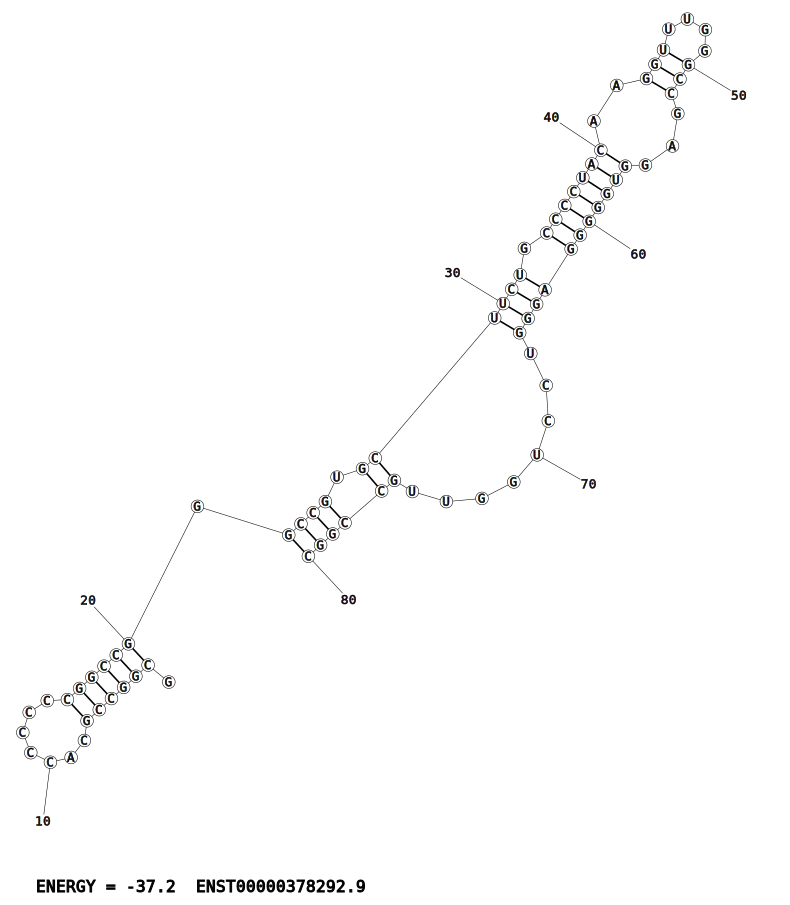
\includegraphics[width=\textwidth]{images/rna-structure/shared-isoforms/ENST00000378292.9.pdf}
  \caption{}
\end{subfigure}
\hfill
\begin{subfigure}{0.48\textwidth}
  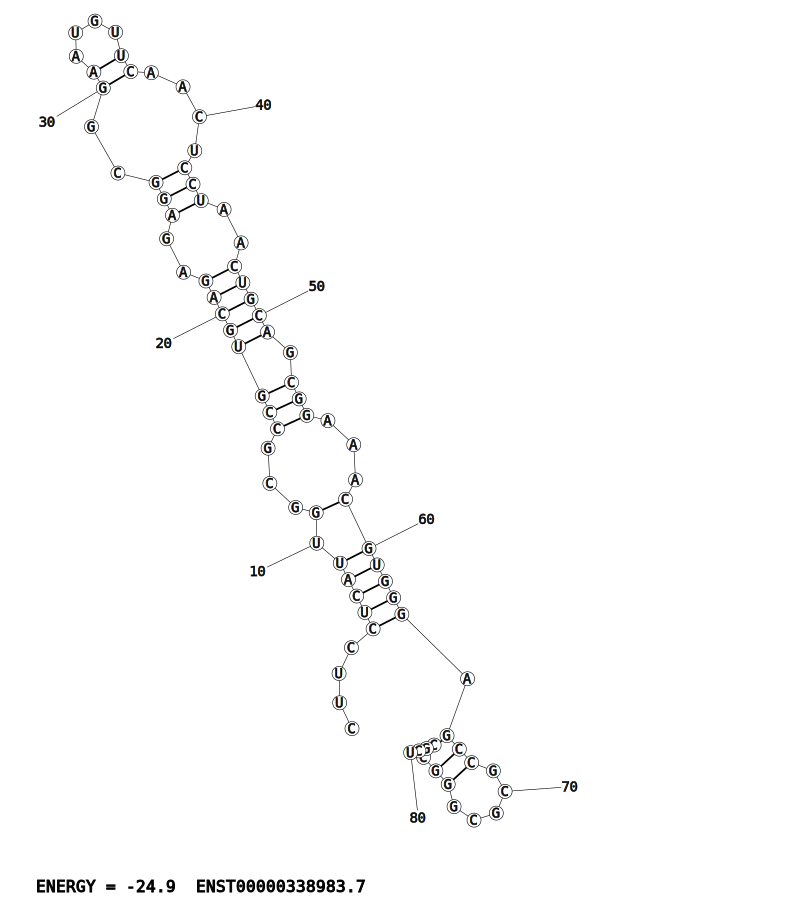
\includegraphics[width=\textwidth]{images/rna-structure/shared-isoforms/ENST00000338983.7.pdf}
  \caption{}
\end{subfigure}

\medskip

\begin{subfigure}{0.48\textwidth}
  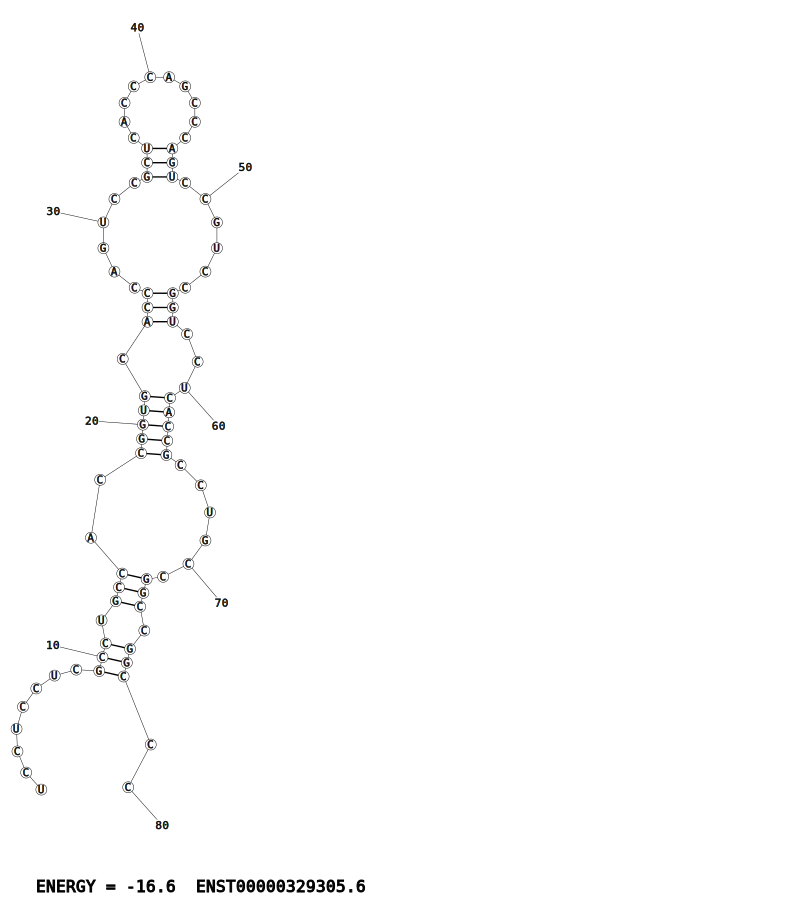
\includegraphics[width=\textwidth]{images/rna-structure/shared-isoforms/ENST00000329305.6.pdf}
  \caption{}
\end{subfigure}
\hfill
\begin{subfigure}{0.48\textwidth}
  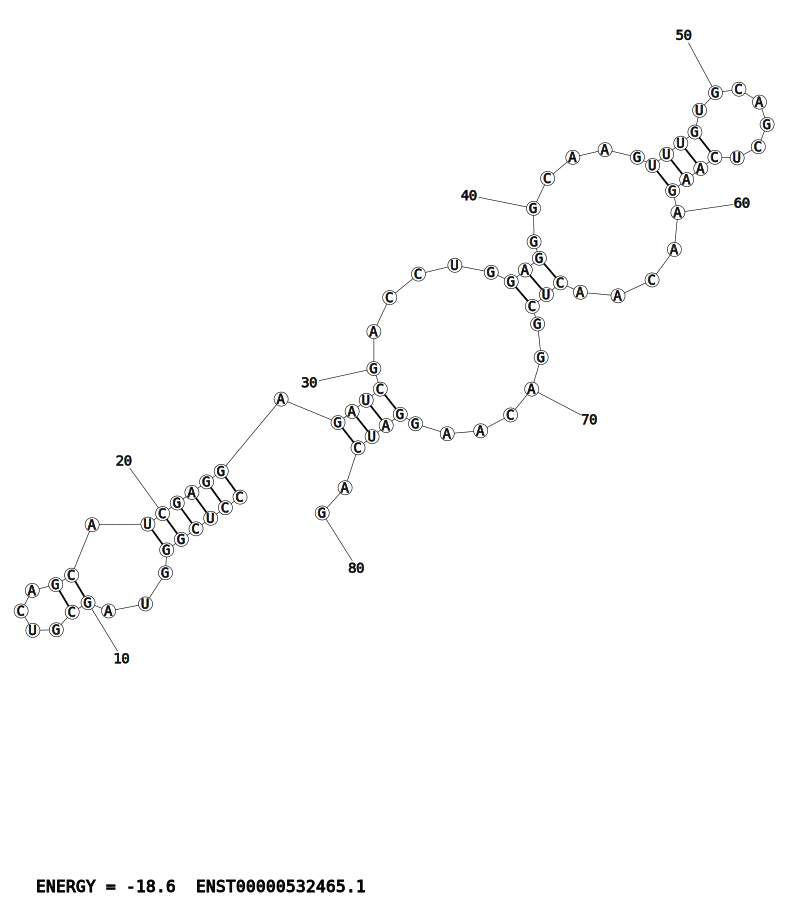
\includegraphics[width=\textwidth]{images/rna-structure/shared-isoforms/ENST00000532465.1.pdf}
  \caption{}
\end{subfigure}

\caption{RNA secondary structure prediction of isoforms shared between EOCRC and LOCRC obtained using \textit{RNAStructure} software. (a) \textit{ENST00000378292.9}, (b) \textit{ENST00000338983.7}, (c) \textit{ENST00000329305.6}, and (d) \textit{ENST00000532465.1}.}
\label{fig:rna_structure_shared_isoforms}
\end{figure}

% Continue - RNA secondary structure prediction of 6 isoforms shared between EOCRC and LOCRC samples

\begin{figure}[!ht]
\centering

\begin{subfigure}{0.48\textwidth}
  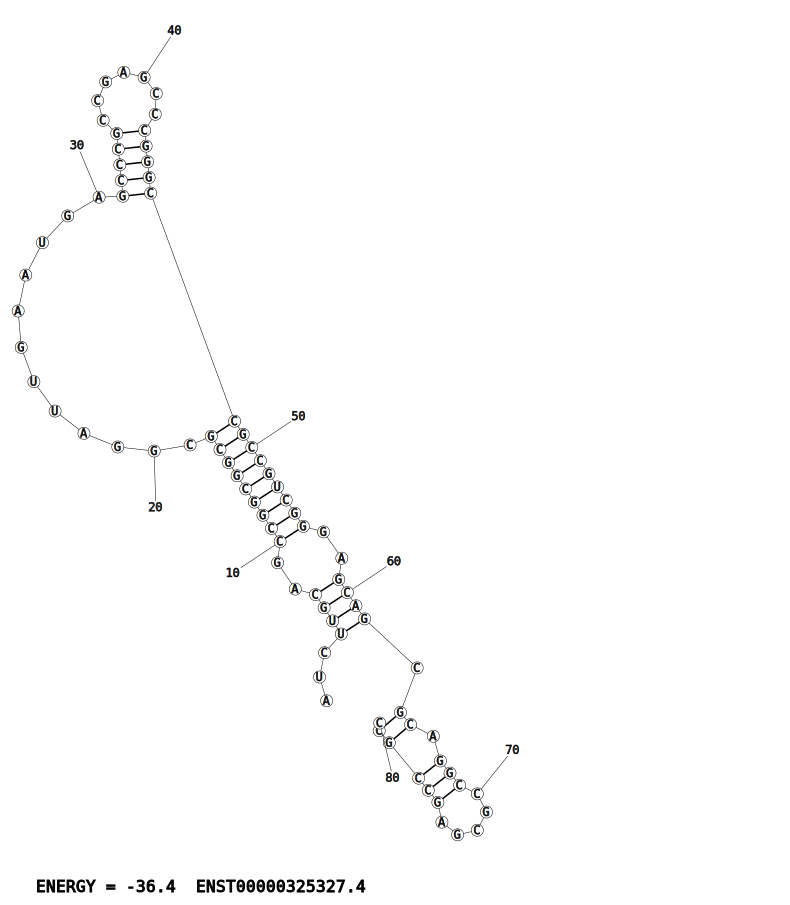
\includegraphics[width=\textwidth]{images/rna-structure/shared-isoforms/ENST00000325327.4.pdf}
  \caption{}
\end{subfigure}
\hfill
\begin{subfigure}{0.48\textwidth}
  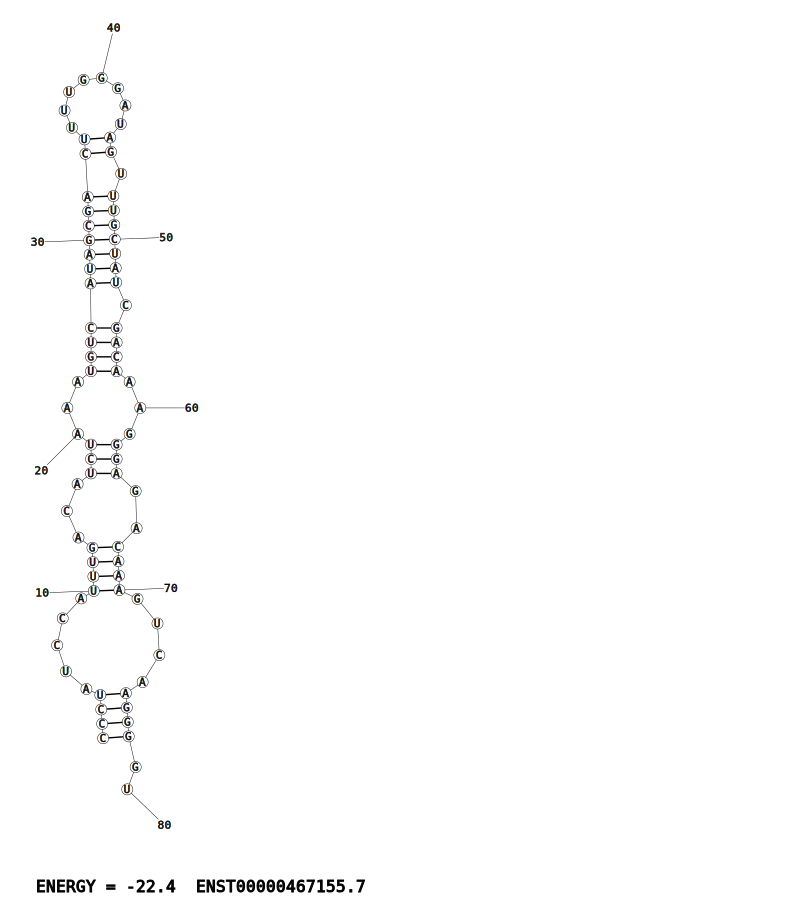
\includegraphics[width=\textwidth]{images/rna-structure/shared-isoforms/ENST00000467155.7.pdf}
  \caption{}
\end{subfigure}

\medskip

\begin{subfigure}{0.48\textwidth}
  \centering
  \includegraphics[width=\textwidth]{images/rna-structure/shared-isoforms/heatmap_structural_elements_6_isoforms-1.pdf}
  \caption{}
\end{subfigure}

\caption{RNA secondary structure prediction of isoforms shared between EOCRC and LOCRC obtained using \textit{RNAStructure} software. (a) \textit{ENST00000325327.4}, (b) \textit{ENST00000467155.7}, and (c) heatmap of RNA secondary structure motifs of the 6 shared DTU isoforms obtained using the \textit{bpRNA} toolkit.}
\label{fig:rna_structure_shared_isoforms_continue}
\end{figure}

%-----------------------------------------------------------

% heatmap plot of RNA secondary structure motifs - EOCRC and LOCRC samples

\begin{figure}[!ht]
\centering

\begin{subfigure}{\textwidth}
  \centering
  \begin{adjustbox}{max height=0.4\textheight}
    \includegraphics[width=\textwidth]{images/rna-structure/EOCRC/heatmap_structural_elements_EOCRC-1.pdf}
  \end{adjustbox}
  \caption{}
\end{subfigure}

\medskip

\begin{subfigure}{\textwidth}
  \centering
  \begin{adjustbox}{max height=0.4\textheight}
    \includegraphics[width=\textwidth]{images/rna-structure/LOCRC/heatmap_structural_elements_LOCRC-1.pdf}
  \end{adjustbox}
  \caption{}
\end{subfigure}

\caption{Heatmap of RNA secondary structure motifs of the top DTU isoforms obtained using the \textit{bpRNA} toolkit. (a) EOCRC samples. (b) LOCRC samples.}
\label{fig:heatmap_structural_elements_eocrc_locrc}
\end{figure}


\chapter{Discussion}
In this work, we analyzed RNA sequencing data from patient-matched tumor and adjacent normal tissues obtained from EOCRC (n = 21) and LOCRC (n = 22) cohorts. While we identified several molecular features associated with EOCRC, including differences in gene expression, isoform usage, and alternative splicing patterns, consistent with prior reports \cite{luMolecularCharacteristicsMicrosatellite2023, marxIdentificationDifferentiallyExpressed2024}, we did not observe broad transcriptome-wide differences distinguishing EOCRC from LOCRC.

\section{Differential Gene Expression Analysis}

Differential gene expression analysis using \textit{DESeq2} identified 40 genes uniquely deregulated in EOCRC. Functional enrichment analysis of these genes revealed overrepresentation of immune-related, inflammatory regulatory, and cell adhesion processes, in agreement with previous transcriptomic studies of EOCRC \cite{gardnerDistinctInnateImmune2021, duIntegratedMultiomicsApproach2023a}. The partial overlap between our 40-gene set and the 48 EOCRC-specific genes identified by Marx et al. \cite{marxIdentificationDifferentiallyExpressed2024} is because we did not apply an additional expression cutoff threshold of 1.5 LFC difference between EOCRC and LOCRC cohorts.

Although clinical and demographic variables were not explicitly modeled in our analysis, despite their known contribution to EOCRC risk \cite{kongIntegratedMetagenomicMetabolomic2023, zhengComprehensiveAssessmentDiet2021}, we nonetheless recovered 4 of the 8 EOCRC-associated gene signatures curated by Marx et al. \cite{marxIdentificationDifferentiallyExpressed2024}. While WNT11, MSLN, and IL1RN have known roles in CRC, SLC38A11 is an understudied candidate in this context. These four genes might give insight into EOCRC pathogenesis and serve as prognostic markers compared to LOCRC based on the following information: 

\begin{itemize}
    \item \textbf{WNT11:} Activates non-canonical Wnt signaling pathways that regulate cell motility and invasion in colorectal cancer \cite{gorrono-etxebarriaWnt11PotentialPrognostic2019}. More recently, circulating WNT11 levels have been proposed as a minimally invasive biomarker for monitoring colorectal cancer liver metastases in the context of immunotherapy \cite{jiangWNT11PromotesImmune2025}.

    \item \textbf{MSLN:} Its high expression in colorectal cancer is associated with immune-related features, including increased macrophage infiltration, elevated PD-L1 levels, and activation of inflammatory signaling pathways \cite{mallaMesothelinExpressionCorrelates2024}. These tumors also frequently harbor KRAS and FBXW7 mutations, suggesting a link between MSLN expression, tumor progression, and immune modulation.

    \item \textbf{IL1RN:} Encodes the interleukin-1 receptor antagonist, a modulator of IL-1 driven inflammation in the tumor microenvironment. Disruptions in \texttt{IL-1/IL-1RN} balance are implicated in cancer-associated inflammation and immune suppression \cite{mantovaniIL1IL1Regulatory2018}. Moreover, IL1RN expression has been reported as a prognostic marker correlated with immune cell infiltration in colorectal cancer \cite{wangIL1RNPRRX1Prognostic2022}.

    \item \textbf{SLC38A11:} A gene implicated in cellular metabolic processes \cite{garrettEarlyonsetColorectalCancer2022}, which has been significantly associated with metastatic progression in colorectal cancer \cite{marxIdentificationDifferentiallyExpressed2024}, suggesting potential clinical relevance in EOCRC patients.
\end{itemize}

\section{Differential Transcript Usage Analysis}

The direct comparison of the alternative splicing analysis conducted by Marx et al. \cite{marxIdentificationDifferentiallyExpressed2024} and our isoform-switch analysis on the same dataset, revealed that these are complementary approaches. Their splice analysis strategy with rMATS and Whippet identified a broad spectrum of splicing perturbations. In contrast, our DTU analysis with \texttt{IsoformSwitchAnalyzeR}, curated these events into a list of significant consequential isoform switches. This indicates that while splicing dysregulation is widespread in CRC, only a subset of these events led to a rewiring of the dominant gene isoform.

Moreover, we observed no overlapping between genes identified by our differential gene expression (DGE) and differential transcript usage (DTU), and event-based splicing analyses from Marx et al. \cite{marxIdentificationDifferentiallyExpressed2024} in both EOCRC and LOCRC cohorts. The absence of shared genes reveals that these analytical layers capture distinct aspects of transcriptome variation. This independence aligns with the understanding that changes in gene level expression profiles, isoform level expression profiles, and alternative splicing events can occur separately \cite{zhangIsoformLevelExpression2013, merinoBenchmarkingWorkflowsDetecting2019, innesGeneExpressionAlternative2024}. Taken together, these findings imply that analyses limited to a single transcriptomic level risk missing relevant molecular changes in colorectal cancer.

Our DTU analysis identified several genes with consistent isoform switching in both EOCRC and LOCRC cohorts, with potential relevance to colorectal cancer biology:

\begin{itemize}
    \item \textbf{TPM2:} It was significantly downregulated at the transcript level in tumors compared with normal tissue in both EOCRC and LOCRC. While direct mechanistic evidence for TPM2 in colorectal cancer remains limited, elevated TPM2 expression in tumor-associated stromal cells was shown to outperform several established prognostic markers, indicating potential clinical relevance for patient stratification \cite{meleIdentificationTPM2CNN12022}.

    \item \textbf{LMNB2:} Functional evidence indicates that LMNB2 promotes tumor cell proliferation by regulating cell cycle progression through the p21 pathway, supporting its relevance as a prognostic marker in CRC \cite{dongLMNB2PromotesProgression2021}.

    \item \textbf{HOXB-AS3:} A lncRNA that encodes a conserved micropeptide that suppresses colorectal cancer growth by modulating alternative splicing of PKM and limiting metabolic reprogramming. Loss of the HOXB-AS3 peptide is associated with increased tumor progression and poorer prognosis in CRC patients \cite{huangPeptideEncodedPutative2017}.

    \item \textbf{MAP3K20:} There is currently no primary literature linking MAP3K20 to colorectal tumorigenesis. However, Marx et al. \cite{marxIdentificationDifferentiallyExpressed2024} identified tumor-specific splicing of a similar gene, MAP3K8 in EOCRC. Both genes belong to the larger Mitogen-Activated Protein Kinase (MAPK) pathway and function as MAP kinase kinase kinases (MAP3Ks). This suggests that dysregulation of MAP3K family members may contribute to CRC pathogenesis.
\end{itemize}

\section{Alternative Splicing Regulation}

Alternative splicing has been proposed as an important regulatory layer contributing to age-related differences in colorectal cancer. Marx et al. \cite{marxIdentificationDifferentiallyExpressed2024} reported a higher number of differentially spliced events in LOCRC compared to EOCRC, with exon skipping representing the dominant splicing category in both cohorts, but with substantially greater complexity in late-onset tumors. In addition, their observation that tumor and normal samples could be separated based on splice junction usage suggests that alternative splicing contributes to the transcriptomic differences between EOCRC and LOCRC.

Our results, obtained through DTU analysis, are consistent with these observations and extend them at the isoform level. While the analytical frameworks differ, both approaches agree that LOCRC tumors exhibit a more extensive splicing perturbation than EOCRC tumors. In our analysis, exon skipping, alternative splice site usage, and other transcript-level alterations affected a higher number of isoforms in LOCRC, whereas EOCRC tumors showed only limited involvement across all splicing categories. 

\section{RNA Secondary Structure Analysis}

Canonical RNA secondary structures including hairpins, stems, bulges, internal loops, and loops are fundamental determinants of RNA function \cite{caoIdentificationRNAStructures2024}, representing an additional regulatory layer beyond nucleotide sequence and gene level expression. In our study, We extended our DTU analysis to examine the RNA secondary structure of key isoforms, asking whether structural differences could distinguish EOCRC from LOCRC transcriptomes.

While we observed a general enrichment of stem motifs across isoforms, a cohort-specific structural signature was not identified. This was because we used little data to make these predictions. Nonetheless, this work provides a necessary framework for future, large-scale studies. This is critical because secondary structure can be a direct target for intervention. For instance, Liu et al. \cite{liuAnalysisSecondaryStructural2016} demonstrated that specific motifs in microRNA precursors provide a rationale for designing small molecules to interfere with their maturation, a strategy that could be adapted to target oncogenic isoforms in CRC. Thus, our pipeline lays the groundwork for identifying such targetable structures in crc-associated transcripts.

\chapter{Conclusions and future works}

Our study implemented an integrative transcriptomic framework to characterize molecular differences between early-onset and late-onset colorectal cancer, combining differential gene expression, differential transcript usage, and RNA secondary structure prediction. This multi-layered approach revealed age-associated heterogeneity that is not captured by gene-level analyses alone. 

A central finding was the identification of a 40-gene signature uniquely deregulated in EOCRC, mainly enriched in immune-related processes. The involvement of genes such as WNT11, MSLN, IL1RN, and SLC38A11 supported the existence of a distinct molecular and immune microenvironment in early-onset disease.

Isoform-level analysis uncovered pronounced differences in post-transcriptional regulation between cohorts. Late-onset tumors exhibited extensive transcriptome remodeling with hundreds of isoform switches, whereas early-onset tumors showed a comparatively constrained splicing landscape. Despite these global differences, six recurrent isoform switches were shared between cohorts, including TPM2, LMNB2, MAP3K20, and the long non-coding RNA HOXB-AS3.

RNA secondary structure prediction revealed a general enrichment of stem motifs among significant isoforms, establishing a computational pipeline for incorporating structural features into transcriptomic analyses. Although age-specific structural signatures were not conclusively identified, this framework provides a foundation for future large-scale studies. 

Overall, the results demonstrate that integrative bioinformatics strategies are essential for capturing transcriptomic complexity and highlight potential molecular candidates relevant to early detection and personalized therapeutic approaches in colorectal cancer.

\section{Planning Follow-up}

The execution of this project faced several technical and methodological challenges that required continuous monitoring and adaptive decision-making. Progress was tracked against predefined milestones using a dedicated GitHub project board, which enabled transparent documentation of changes in scope and analytical strategy. A major risk identified during development was the infeasibility of deploying RiNALMo, an RNA large language models for secondary structure prediction, due to GPU memory and architecture constraints on the available infrastructure at the University of Navarra. This limitation necessitated a revision of the original project scope and a methodological pivot toward thermodynamics-based RNA structure prediction using \textit{RNAStructure}. Additional risks related to biological interpretability were mitigated by anchoring downstream structural analyses to high-confidence candidates derived from differential gene expression and differential transcript usage analyses. These mitigation strategies ensured that, despite infrastructure constraints and analytical complexity, all core objectives were achieved within the planned timeline.

\section{Improvements and Future Work}

As future work, we propose to perform differential transcript usage analysis using the \href{https://nf-co.re/rnasplice/dev/}{nf-core/rnasplice} pipeline as an alternative to the manual approach based on \texttt{IsoformSwitchAnalyzeR}. This comparison would allow the assessment of result consistency while improving reproducibility through the use of a standardized and community-maintained workflow. The \texttt{nf-core/rnasplice} pipeline is a relatively recent tool whose adoption has steadily increased, making it a robust option for large-scale alternative splicing analyses.

The combined use of multiple \texttt{Nextflow}-based pipelines enables the coherent integration of differential gene expression (DGE) and differential transcript usage (DTU) analyses. In this context, a relevant improvement would be the automation of nucleotide sequence extraction from the most significant isoform switches, followed by the incorporation of an additional module for RNA secondary structure prediction. Since \texttt{Nextflow} constitutes the core processing framework, this integration could be implemented through auxiliary scripts, such as \texttt{Bash} or \texttt{Python}, allowing the construction of a unified workflow encompassing DGE, DTU, and RNA secondary structure analyses.

Furthermore, the current workflow could be extended by incorporating public RNA-seq data from one of the most comprehensive studies conducted to date in colorectal cancer, \emph{Prognostic genome and transcriptome signatures in colorectal cancers}~\cite{nunesPrognosticGenomeTranscriptome2024}. This study includes RNA-seq data from 1183 colorectal cancer patients. The main objective of this extension would be to identify a larger number of isoform switches, particularly involving non-coding RNAs, with potential value as biomarkers for early-onset colorectal cancer, thereby contributing to a deeper understanding of the molecular mechanisms underlying disease pathogenesis.

Finally, future efforts could focus on exploring state-of-the-art computational approaches, such as large language models for RNA such as RiNALMo, whose application to RNA secondary structure prediction has recently gained significant attention within the scientific community. In this context, we aim to reproduce and integrate methodologies described in recent benchmarking studies, such as \emph{Comprehensive benchmarking of large language models for RNA secondary structure prediction}~\cite{zablockiComprehensiveBenchmarkingLarge2025}, once access to the computational infrastructure provided by the EuroCC Spain Testbed becomes available.

%-----------------------------------------------------------

\chapter{Glossary}

\begin{description}

\item[Colorectal Cancer (CRC)] One of the leading causes of global cancer-related mortality and morbidity, traditionally associated with older populations.

\item[Early-Onset Colorectal Cancer (EOCRC)] A subtype of colorectal cancer diagnosed in individuals younger than 50 years, often exhibiting distinct clinical, molecular, and prognostic characteristics.

\item[Late-Onset Colorectal Cancer (LOCRC)] Colorectal cancer diagnosed in individuals older than 50 years, used in this study as a reference cohort for identifying age-associated molecular differences.

\item[Transcriptome] The complete set of RNA transcripts produced by the genome, commonly analyzed using RNA sequencing to identify dysregulated pathways and candidate biomarkers.

\item[Differential Gene Expression (DGE)] A statistical analysis used to identify genes with significant changes in overall expression levels between biological conditions, such as tumor and normal tissues.

\item[Differential Transcript Usage (DTU)] An analytical approach that detects changes in the relative usage of transcript isoforms between conditions, independent of total gene expression.

\item[Alternative Splicing] A post-transcriptional regulatory mechanism that produces multiple mRNA isoforms from a single gene, contributing to functional and proteomic diversity.

\item[Isoform Switch] An event in which the dominant transcript isoform of a gene differs between biological conditions, potentially altering gene function.

\item[RNA Secondary Structure (RSS)] The two-dimensional folding patterns adopted by RNA molecules, which influence their stability, interactions, and biological function beyond nucleotide sequence.

\item[Minimum Free Energy (MFE)] A thermodynamic principle used in computational RNA folding to predict the most stable RNA conformation.

\item[Pseudo-alignment] A computational method for estimating transcript abundance by mapping sequencing reads to a transcriptome index rather than performing full genomic alignment.

\item[Gene Ontology (GO) Enrichment] A statistical method used to identify biological processes, molecular functions, or cellular components that are overrepresented in a given gene set.

\item[Structural Motifs] Discrete elements of RNA secondary structure, including stems, hairpins, bulges, and internal loops, used to characterize RNA structural complexity.

\item[Long Non-coding RNA (lncRNA)] RNA transcripts longer than 200 nucleotides that do not encode proteins but play important regulatory roles in gene expression and cellular processes.

\end{description}

%-----------------------------------------------------------

\bibliographystyle{unsrt}
\bibliography{references}


%\newpage
\appendix

\chapter{EOCRC supplementary figures and tables}
\label{app:eocrc_complementary_results}

%---------------------------------------------------------

% untransformed and log2 transformed counts - EOCRC samples

\begin{figure}[!htbp]
\centering

\begin{subfigure}{\textwidth}
  \includegraphics[width=\textwidth]{images/dge/EOCRC/normal_log2_transformed_counts-1.pdf}
  \caption{}
\end{subfigure}

\medskip

\begin{subfigure}{\textwidth}
  \includegraphics[width=\textwidth]{images/dge/EOCRC/normal_log2_transformed_counts-2.pdf}
  \caption{}
\end{subfigure}

\caption{EOCRC samples (a) Normalized counts before log2 transformation. (b) Normalized counts after log2 transformation.}
\label{app:normal_log2_transformed_counts_eocrc}
\end{figure}

%-----------------------------------------------------------

\begin{figure}[!htbp]
     \centering
     \includegraphics[width=\textwidth]{images/dge/EOCRC/normalization_transformation_summary_counts-1.pdf}
     \caption{Comparison of different normalization and data transformation methods for EOCRC samples. (a) Raw counts before normalization. (b) Normalized counts after sequencing depth normalization. (c) Normalized counts after variance stabilizing transformation (vst). (d) Normalized counts after regularized log transformation (rlog).}
     \label{app:normalization_transformation_summary_counts_eocrc}
\end{figure}

%---------------------------------------------------------
\begin{figure}[htbp]
\centering

\begin{subfigure}{0.48\textwidth}
  \includegraphics[width=\textwidth]{images/dge/EOCRC/pca_condition_tissue_age_stage-1.pdf}
  \caption{}
\end{subfigure}
\hfill
\begin{subfigure}{0.48\textwidth}
  \includegraphics[width=\textwidth]{images/dge/EOCRC/pca_condition_tissue_age_stage-2.pdf}
  \caption{}
\end{subfigure}

\medskip

\begin{subfigure}{\textwidth}
  \centering
  \includegraphics{images/dge/EOCRC/pca_condition_tissue_age_stage-3.pdf}
  \caption{}
\end{subfigure}

\caption{PCA of EOCRC samples based on \texttt{condition \& tissue, condition \& tissue \& age at surgery, condition \& tumor stage}.}
\label{app:pca_condition_tissue_age_stage_eocrc}
\end{figure}

%-----------------------------------------------------------
% Distance heatmap plot - EOCRC samples
\begin{figure}[!ht]
     \centering
     \includegraphics[width=\textwidth]{images/dge/EOCRC/distance_pheatmap-1.pdf}
     \caption{Distance heatmap of EOCRC samples based on variance stabilizing transformation (vst) normalized counts. The heatmap displays hierarchical clustering of samples, with color intensity representing the distance between sample expression profiles.}
     \label{app:distance_pheatmap_eocrc}
\end{figure}

%---------------------------------------------------------

\begin{figure}[!htbp]
     \centering
     \includegraphics[width=\textwidth]{images/dge/EOCRC/hierachical_pheatmap-1.pdf}
     \caption{Hierachical heatmap of EOCRC samples.}
     \label{app:hierachical_pheatmap_eocrc}
\end{figure}

%---------------------------------------------------------

% Top differentially expressed genes (DEGs) table of the EOCRC cohort
\begin{table}[!ht]
\centering
\caption{Top DEGs of the EOCRC cohort.}
\begin{adjustbox}{width=0.8\textwidth}
  
\begin{tabular}{llrrl}
\toprule
  & Gene & baseMean & log2FoldChange & padj\\
\midrule
ENSG00000105464 & GRIN2D & 140.9 & 4.173 & 1.92e-27\\
ENSG00000164283 & ESM1 & 109.8 & 5.233 & 1.32e-26\\
ENSG00000175832 & ETV4 & 726.7 & 4.371 & 5.78e-24\\
ENSG00000107159 & CA9 & 388.8 & 5.637 & 1.03e-20\\
ENSG00000163347 & CLDN1 & 625.0 & 4.503 & 1.03e-20\\
ENSG00000170373 & CST1 & 396.6 & 7.035 & 1.03e-20\\
ENSG00000172031 & EPHX4 & 75.8 & 4.433 & 1.03e-20\\
ENSG00000236081 & ELFN1-AS1 & 137.8 & 4.789 & 1.03e-20\\
ENSG00000111110 & PPM1H & 322.7 & 2.141 & 1.36e-20\\
ENSG00000172164 & SNTB1 & 362.7 & 2.083 & 3.14e-20\\
ENSG00000108244 & KRT23 & 683.8 & 6.429 & 6.29e-20\\
ENSG00000181577 & LINC03040 & 230.7 & 4.475 & 1.71e-19\\
ENSG00000178773 & CPNE7 & 219.2 & 4.129 & 2.29e-19\\
ENSG00000164379 & FOXQ1 & 402.9 & 4.316 & 8.63e-19\\
ENSG00000143412 & ANXA9 & 57.7 & 4.183 & 3.24e-18\\
ENSG00000101255 & TRIB3 & 475.7 & 3.205 & 4.92e-18\\
ENSG00000006071 & ABCC8 & 18.9 & -3.287 & 6.02e-18\\
ENSG00000015413 & DPEP1 & 2447.4 & 5.143 & 1.27e-17\\
ENSG00000050344 & NFE2L3 & 1521.0 & 2.459 & 1.85e-17\\
ENSG00000162073 & PAQR4 & 567.1 & 2.020 & 1.93e-17\\
ENSG00000100505 & TRIM9 & 55.1 & -3.364 & 6.88e-17\\
ENSG00000171951 & SCG2 & 298.4 & -3.263 & 7.52e-17\\
ENSG00000103021 & CFAP263 & 134.0 & 2.198 & 8.55e-17\\
ENSG00000173894 & CBX2 & 108.6 & 3.503 & 8.62e-17\\
ENSG00000104237 & RP1 & 21.6 & 5.431 & 2.20e-16\\
ENSG00000034971 & MYOC & 22.4 & -4.999 & 2.40e-16\\
ENSG00000281406 & BLACAT1 & 93.9 & 4.173 & 2.61e-16\\
ENSG00000212993 & POU5F1B & 95.9 & 4.010 & 3.62e-16\\
ENSG00000245694 & CRNDE & 65.3 & 3.435 & 5.01e-16\\
ENSG00000129474 & AJUBA & 156.1 & 2.731 & 8.76e-16\\
\bottomrule
\end{tabular}

\end{adjustbox}
\label{app:top_deg_eocrc}
\end{table}

%-----------------------------------------------------------
\chapter{LOCRC supplementary figures and tables}
\label{app:locrc_complementary_results}

%---------------------------------------------------------
\begin{figure}[!htbp]
\centering

\begin{subfigure}{\textwidth}
  \includegraphics[width=\textwidth]{images/dge/LOCRC/normal_log2_transformed_counts-1.pdf}
  \caption{}
\end{subfigure}

\medskip

\begin{subfigure}{\textwidth}
  \includegraphics[width=\textwidth]{images/dge/LOCRC/normal_log2_transformed_counts-2.pdf}
  \caption{}
\end{subfigure}

\caption{LOCRC samples (a) Normalized counts before log2 transformation. (b) Normalized counts after log2 transformation.}
\label{app:normal_log2_transformed_counts}
\end{figure}

%-----------------------------------------------------------

\begin{figure}[!htbp]
     \centering
     \includegraphics[width=\textwidth]{images/dge/LOCRC/normalization_transformation_summary_counts-1.pdf}
     \caption{Comparison of different normalization and data transformation methods for LOCRC samples. (a) Raw counts before normalization. (b) Normalized counts after sequencing depth normalization. (c) Normalized counts after variance stabilizing transformation (vst). (d) Normalized counts after regularized log transformation (rlog).}
     \label{app:normalization_transformation_summary_counts}
\end{figure}

%---------------------------------------------------------
\begin{figure}[htbp]
\centering

\begin{subfigure}{0.48\textwidth}
  \includegraphics[width=\textwidth]{images/dge/LOCRC/pca_condition_tissue_age_stage-1.pdf}
  \caption{}
\end{subfigure}
\hfill
\begin{subfigure}{0.48\textwidth}
  \includegraphics[width=\textwidth]{images/dge/LOCRC/pca_condition_tissue_age_stage-2.pdf}
  \caption{}
\end{subfigure}

\medskip

\begin{subfigure}{\textwidth}
  \centering
  \includegraphics{images/dge/LOCRC/pca_condition_tissue_age_stage-3.pdf}
  \caption{}
\end{subfigure}

\caption{PCA of LOCRC samples based on \texttt{condition \& tissue, condition \& tissue \& age at surgery, condition \& tumor stage}.}
\label{app:pca_condition_tissue_age_stage_locrc}
\end{figure}

%---------------------------------------------------------

% Distance heatmap plot - LOCRC samples
\begin{figure}[!ht]
     \centering
     \includegraphics[width=\textwidth]{images/dge/LOCRC/distance_pheatmap-1.pdf}
     \caption{Distance heatmap of LOCRC samples based on variance stabilizing transformation (vst) normalized counts. The heatmap displays hierarchical clustering of samples, with color intensity representing the distance between sample expression profiles.}
     \label{app:distance_pheatmap_locrc}
\end{figure}
%-----------------------------------------------------------

\begin{figure}[!htbp]
     \centering
     \includegraphics[width=\textwidth]{images/dge/LOCRC/hierachical_pheatmap-1.pdf}
     \caption{Hierachical heatmap of LOCRC samples.}
     \label{app:hierachical_pheatmap_locrc}
\end{figure}

%---------------------------------------------------------

% Top differentially expressed genes (DEGs) table of the LOCRC cohort
\begin{table}[!ht]
\centering
\caption{Top DEGs of the LOCRC cohort.}
\begin{adjustbox}{width=0.8\textwidth}
  
\begin{tabular}{llrrl}
\toprule
  & Gene & baseMean & log2FoldChange & padj\\
\midrule
ENSG00000175832 & ETV4 & 777.7 & 5.908 & 6.42e-100\\
ENSG00000164379 & FOXQ1 & 554.6 & 6.813 & 3.43e-68\\
ENSG00000173898 & SPTBN2 & 335.2 & 3.844 & 1.42e-61\\
ENSG00000287828 & NA & 117.9 & 3.743 & 2.31e-55\\
ENSG00000111110 & PPM1H & 475.6 & 2.841 & 8.86e-53\\
ENSG00000165816 & VWA2 & 447.5 & 4.612 & 4.59e-49\\
ENSG00000164283 & ESM1 & 72.8 & 5.750 & 2.78e-48\\
ENSG00000015413 & DPEP1 & 1834.3 & 6.596 & 1.12e-47\\
ENSG00000120708 & TGFBI & 8131.2 & 2.903 & 1.07e-46\\
ENSG00000162073 & PAQR4 & 378.3 & 1.920 & 1.99e-45\\
ENSG00000214039 & LINC02418 & 301.2 & 8.239 & 3.19e-45\\
ENSG00000186462 & NAP1L2 & 52.1 & -3.451 & 4.65e-45\\
ENSG00000183734 & ASCL2 & 740.2 & 4.241 & 5.55e-45\\
ENSG00000172031 & EPHX4 & 78.0 & 5.329 & 1.47e-43\\
ENSG00000163347 & CLDN1 & 850.1 & 4.858 & 4.30e-43\\
ENSG00000165905 & LARGE2 & 185.1 & 4.659 & 4.30e-43\\
ENSG00000128059 & PPAT & 488.3 & 2.212 & 1.28e-41\\
ENSG00000071539 & TRIP13 & 299.5 & 2.990 & 2.43e-41\\
ENSG00000281406 & BLACAT1 & 105.6 & 5.527 & 5.36e-40\\
ENSG00000171617 & ENC1 & 2115.8 & 2.004 & 1.75e-39\\
ENSG00000219481 & NBPF1 & 1163.8 & -2.384 & 3.03e-39\\
ENSG00000103494 & RPGRIP1L & 191.4 & 2.022 & 6.73e-39\\
ENSG00000103888 & CEMIP & 1134.0 & 4.976 & 8.27e-39\\
ENSG00000165376 & CLDN2 & 971.6 & 7.699 & 1.08e-38\\
ENSG00000120254 & MTHFD1L & 472.9 & 2.701 & 1.74e-38\\
ENSG00000169247 & SH3TC2 & 174.7 & 3.959 & 2.01e-38\\
ENSG00000185269 & NOTUM & 222.7 & 8.730 & 2.83e-38\\
ENSG00000103021 & CFAP263 & 136.9 & 2.115 & 3.03e-38\\
ENSG00000105948 & IFT56 & 137.2 & 2.313 & 4.40e-38\\
ENSG00000123643 & SLC36A1 & 1170.9 & -2.367 & 6.16e-38\\
\bottomrule
\end{tabular}

\end{adjustbox}
\label{app:top_deg_locrc}
\end{table}

%-----------------------------------------------------------
\chapter{DTU analysis supplementary data}
\label{app:dtu_complementary_results}

\small 
\begin{longtable}{l l l l r r r}
\caption{Top isoforms from each comparison
\texttt{normal\_eocrc vs tumor\_eocrc and normal\_locrc vs tumor\_locrc} ordered by \texttt{q-value}.} \\
\label{tab:top_isoforms_from_each_comparison} \\

\toprule
Isoform ID & Gene ID & Condition 1 & Condition 2 & dIF & q-value & Rank \\
\midrule
\endfirsthead

\multicolumn{7}{c}{\textbf{Table \thetable\ (continued from previous page)}} \\
\toprule
Isoform ID & Gene ID & Condition 1 & Condition 2 & dIF & q-value & Rank \\
\midrule
\endhead

\midrule
\multicolumn{7}{r}{Continued on next page} \\
\endfoot

\bottomrule
\endlastfoot

ENST00000378292.9 & TPM2 & normal\_eocrc & tumor\_eocrc & -0.133 & 0.0001117 & 1\\
ENST00000698539.1 & SORBS2 & normal\_locrc & tumor\_locrc & -0.233 & 0.0001545 & 2\\
ENST00000378292.9 & TPM2 & normal\_locrc & tumor\_locrc & -0.173 & 0.0001545 & 3\\
ENST00000642527.1 & FSIP1 & normal\_locrc & tumor\_locrc & 0.112 & 0.0001622 & 4\\
ENST00000319481.8 & OSBPL1A & normal\_locrc & tumor\_locrc & 0.294 & 0.0002382 & 5\\
ENST00000338983.7 & MAP3K20 & normal\_locrc & tumor\_locrc & -0.273 & 0.0003502 & 6\\
ENST00000263398.11 & CD44 & normal\_locrc & tumor\_locrc & -0.311 & 0.0004923 & 7\\
ENST00000374429.6 & CXCL12 & normal\_locrc & tumor\_locrc & 0.214 & 0.0006191 & 8\\
ENST00000865845.1 & NLN & normal\_locrc & tumor\_locrc & 0.203 & 0.0006191 & 9\\
ENST00000316673.9 & HNF4A & normal\_locrc & tumor\_locrc & 0.408 & 0.0009308 & 10\\
ENST00000637069.1 & KIAA1671 & normal\_locrc & tumor\_locrc & 0.318 & 0.0016565 & 11\\
ENST00000356861.9 & TNPO2 & normal\_locrc & tumor\_locrc & -0.423 & 0.0016565 & 12\\
ENST00000885410.1 & SESN1 & normal\_locrc & tumor\_locrc & -0.150 & 0.0018008 & 13\\
ENST00000329305.6 & TPM2 & normal\_locrc & tumor\_locrc & 0.115 & 0.0018008 & 14\\
ENST00000373827.6 & ANK3 & normal\_locrc & tumor\_locrc & 0.139 & 0.0019256 & 15\\
ENST00000415602.5 & TCEA2 & normal\_eocrc & tumor\_eocrc & 0.116 & 0.0020556 & 16\\
ENST00000433644.2 & FANCC & normal\_locrc & tumor\_locrc & 0.235 & 0.0020820 & 17\\
ENST00000507460.1 & GABRA2 & normal\_locrc & tumor\_locrc & 0.133 & 0.0020820 & 18\\
ENST00000635823.2 & KIF16B & normal\_locrc & tumor\_locrc & -0.305 & 0.0020820 & 19\\
ENST00000624247.1 & SMTN & normal\_locrc & tumor\_locrc & -0.176 & 0.0022917 & 20\\
ENST00000489337.5 & SMTN & normal\_locrc & tumor\_locrc & 0.076 & 0.0024667 & 21\\
ENST00000329305.6 & TPM2 & normal\_eocrc & tumor\_eocrc & 0.101 & 0.0025112 & 22\\
ENST00000532465.1 & LMNB2 & normal\_locrc & tumor\_locrc & -0.246 & 0.0029059 & 23\\
ENST00000325327.4 & LMNB2 & normal\_locrc & tumor\_locrc & 0.232 & 0.0029544 & 24\\
ENST00000367514.7 & C1orf21 & normal\_locrc & tumor\_locrc & 0.337 & 0.0030037 & 25\\
ENST00000454658.6 & SINHCAF & normal\_locrc & tumor\_locrc & -0.101 & 0.0030037 & 26\\
ENST00000412051.5 & CHLSN & normal\_locrc & tumor\_locrc & -0.269 & 0.0031328 & 27\\
ENST00000393414.6 & IL1R2 & normal\_locrc & tumor\_locrc & 0.248 & 0.0040455 & 28\\
ENST00000301843.13 & CTTN & normal\_locrc & tumor\_locrc & 0.235 & 0.0041748 & 29\\
ENST00000705474.1 & TNS3 & normal\_locrc & tumor\_locrc & -0.264 & 0.0041748 & 30\\
ENST00000361901.6 & CALD1 & normal\_locrc & tumor\_locrc & 0.277 & 0.0045070 & 31\\
ENST00000316099.10 & HNF4A & normal\_locrc & tumor\_locrc & -0.421 & 0.0045070 & 32\\
ENST00000337130.10 & UGP2 & normal\_locrc & tumor\_locrc & -0.436 & 0.0048100 & 33\\
ENST00000539026.1 & LINC01559 & normal\_eocrc & tumor\_eocrc & -0.160 & 0.0050706 & 34\\
ENST00000382040.4 & RSAD2 & normal\_eocrc & tumor\_eocrc & -0.157 & 0.0050706 & 35\\
ENST00000341723.8 & HEPACAM2 & normal\_locrc & tumor\_locrc & -0.255 & 0.0055968 & 36\\
ENST00000391839.6 & COX20 & normal\_locrc & tumor\_locrc & -0.167 & 0.0057885 & 37\\
ENST00000378943.7 & GK & normal\_locrc & tumor\_locrc & 0.231 & 0.0057931 & 38\\
ENST00000283365.14 & DTNA & normal\_locrc & tumor\_locrc & 0.100 & 0.0060797 & 39\\
ENST00000904832.1 & ACTN1 & normal\_locrc & tumor\_locrc & -0.171 & 0.0061631 & 40\\
ENST00000318426.6 & LINC01559 & normal\_eocrc & tumor\_eocrc & 0.139 & 0.0062714 & 41\\
ENST00000871508.1 & UGT2B15 & normal\_locrc & tumor\_locrc & -0.536 & 0.0069021 & 42\\
ENST00000394468.7 & HEPACAM2 & normal\_locrc & tumor\_locrc & 0.160 & 0.0071537 & 43\\
ENST00000399443.7 & OSBPL1A & normal\_locrc & tumor\_locrc & -0.341 & 0.0071537 & 44\\
ENST00000222902.7 & CCL24 & normal\_locrc & tumor\_locrc & -0.280 & 0.0073466 & 45\\
ENST00000449201.5 & NT5C3A & normal\_locrc & tumor\_locrc & -0.113 & 0.0073466 & 46\\
ENST00000610140.7 & NT5C3A & normal\_locrc & tumor\_locrc & 0.142 & 0.0078493 & 47\\
ENST00000864419.1 & RERE & normal\_locrc & tumor\_locrc & 0.146 & 0.0080275 & 48\\
ENST00000415691.2 & HNF4A & normal\_locrc & tumor\_locrc & -0.056 & 0.0081462 & 49\\
ENST00000373672.8 & COL16A1 & normal\_locrc & tumor\_locrc & -0.204 & 0.0086799 & 50\\
ENST00000570103.5 & CFDP1 & normal\_locrc & tumor\_locrc & -0.324 & 0.0088678 & 51\\
ENST00000560234.1 & PCLAF & normal\_locrc & tumor\_locrc & -0.193 & 0.0088678 & 52\\
ENST00000283882.4 & CFDP1 & normal\_locrc & tumor\_locrc & 0.288 & 0.0088928 & 53\\
ENST00000394417.7 & UGP2 & normal\_locrc & tumor\_locrc & 0.420 & 0.0093767 & 54\\
ENST00000406659.3 & DNMT3A & normal\_locrc & tumor\_locrc & -0.127 & 0.0104062 & 55\\
ENST00000354655.9 & ACSL5 & normal\_locrc & tumor\_locrc & -0.282 & 0.0105226 & 56\\
ENST00000563608.2 & PRMT7 & normal\_locrc & tumor\_locrc & -0.204 & 0.0105784 & 57\\
ENST00000262820.7 & KLHL13 & normal\_locrc & tumor\_locrc & 0.096 & 0.0109470 & 58\\
ENST00000380291.5 & AP1S2 & normal\_locrc & tumor\_locrc & 0.089 & 0.0119636 & 59\\
ENST00000467155.7 & HOXB-AS3 & normal\_locrc & tumor\_locrc & -0.137 & 0.0119636 & 60\\
ENST00000630269.2 & MLLT3 & normal\_locrc & tumor\_locrc & 0.189 & 0.0119636 & 61\\
ENST00000393353.7 & FHL2 & normal\_locrc & tumor\_locrc & 0.116 & 0.0126306 & 62\\
ENST00000490982.1 & TRPM2 & normal\_locrc & tumor\_locrc & 0.422 & 0.0126306 & 63\\
ENST00000216129.7 & TTLL12 & normal\_locrc & tumor\_locrc & 0.337 & 0.0126306 & 64\\
ENST00000866634.1 & UBXN10 & normal\_locrc & tumor\_locrc & 0.327 & 0.0126306 & 65\\
ENST00000305139.11 & UGT1A6 & normal\_locrc & tumor\_locrc & 0.359 & 0.0136912 & 66\\
ENST00000416943.1 & CCL24 & normal\_locrc & tumor\_locrc & 0.210 & 0.0141782 & 67\\
ENST00000859089.1 & KHNYN & normal\_locrc & tumor\_locrc & -0.375 & 0.0141782 & 68\\
ENST00000697576.1 & ZNF44 & normal\_locrc & tumor\_locrc & 0.121 & 0.0141782 & 69\\
ENST00000746568.1 & SPEN-AS1 & normal\_locrc & tumor\_locrc & 0.376 & 0.0141972 & 70\\
ENST00000887088.1 & TNS3 & normal\_locrc & tumor\_locrc & 0.063 & 0.0146668 & 71\\
ENST00000297268.11 & COL1A2 & normal\_eocrc & tumor\_eocrc & 0.193 & 0.0155919 & 72\\
ENST00000532465.1 & LMNB2 & normal\_eocrc & tumor\_eocrc & -0.190 & 0.0163917 & 73\\
ENST00000489749.1 & RSAD2 & normal\_eocrc & tumor\_eocrc & 0.117 & 0.0163917 & 74\\
ENST00000601295.2 & ZNF708 & normal\_locrc & tumor\_locrc & 0.272 & 0.0182954 & 75\\
ENST00000397317.8 & CLDN7 & normal\_locrc & tumor\_locrc & -0.158 & 0.0185549 & 76\\
ENST00000458715.5 & COL16A1 & normal\_locrc & tumor\_locrc & -0.064 & 0.0188584 & 77\\
ENST00000307486.12 & MAB21L4 & normal\_locrc & tumor\_locrc & -0.485 & 0.0190188 & 78\\
ENST00000737891.1 & ENSG00000296299 & normal\_locrc & tumor\_locrc & -0.229 & 0.0201571 & 79\\
ENST00000322142.13 & FHL2 & normal\_locrc & tumor\_locrc & -0.102 & 0.0204909 & 80\\
ENST00000369856.8 & FLNA & normal\_locrc & tumor\_locrc & 0.147 & 0.0207518 & 81\\
ENST00000355288.6 & ANK3 & normal\_locrc & tumor\_locrc & -0.206 & 0.0207739 & 82\\
ENST00000955652.1 & FAM200A & normal\_locrc & tumor\_locrc & -0.347 & 0.0210044 & 83\\
ENST00000851604.1 & SLC39A14 & normal\_locrc & tumor\_locrc & 0.175 & 0.0211065 & 84\\
ENST00000913175.1 & VSNL1 & normal\_locrc & tumor\_locrc & -0.100 & 0.0212544 & 85\\
ENST00000509819.1 & ABLIM2 & normal\_locrc & tumor\_locrc & -0.323 & 0.0217980 & 86\\
ENST00000515595.1 & NLN & normal\_locrc & tumor\_locrc & -0.366 & 0.0217980 & 87\\
ENST00000526995.6 & TRAF6 & normal\_locrc & tumor\_locrc & 0.228 & 0.0217980 & 88\\
ENST00000325327.4 & LMNB2 & normal\_eocrc & tumor\_eocrc & 0.192 & 0.0220051 & 89\\
ENST00000338983.7 & MAP3K20 & normal\_eocrc & tumor\_eocrc & -0.217 & 0.0220051 & 90\\
ENST00000875353.1 & PPARD & normal\_locrc & tumor\_locrc & -0.419 & 0.0225768 & 91\\
ENST00000439587.6 & TMEM8B & normal\_locrc & tumor\_locrc & 0.233 & 0.0230987 & 92\\
ENST00000899612.1 & RAB27A & normal\_locrc & tumor\_locrc & -0.271 & 0.0239662 & 93\\
ENST00000559547.1 & FSIP1 & normal\_locrc & tumor\_locrc & -0.611 & 0.0242630 & 94\\
ENST00000247829.8 & TSPAN8 & normal\_locrc & tumor\_locrc & 0.230 & 0.0243448 & 95\\
ENST00000408042.5 & KIF16B & normal\_locrc & tumor\_locrc & -0.101 & 0.0251548 & 96\\
ENST00000851603.1 & SLC39A14 & normal\_locrc & tumor\_locrc & -0.263 & 0.0260724 & 97\\
ENST00000290079.9 & TMEM141 & normal\_locrc & tumor\_locrc & -0.138 & 0.0261822 & 98\\
ENST00000428004.6 & ABLIM2 & normal\_locrc & tumor\_locrc & 0.167 & 0.0281337 & 99\\
ENST00000301420.3 & KLK1 & normal\_locrc & tumor\_locrc & -0.224 & 0.0285900 & 100\\
ENST00000450644.2 & AP1S2 & normal\_locrc & tumor\_locrc & 0.103 & 0.0293481 & 101\\
ENST00000590247.7 & PDCD5 & normal\_locrc & tumor\_locrc & -0.173 & 0.0298075 & 102\\
ENST00000606752.1 & USP6NL & normal\_locrc & tumor\_locrc & -0.126 & 0.0298075 & 103\\
ENST00000933817.1 & NVL & normal\_locrc & tumor\_locrc & -0.345 & 0.0303730 & 104\\
ENST00000371878.5 & KLHL13 & normal\_locrc & tumor\_locrc & 0.109 & 0.0310361 & 105\\
ENST00000699484.1 & CLCA4-AS1 & normal\_locrc & tumor\_locrc & 0.179 & 0.0311711 & 106\\
ENST00000676000.1 & PURA & normal\_locrc & tumor\_locrc & 0.197 & 0.0311711 & 107\\
ENST00000356644.7 & SESN1 & normal\_locrc & tumor\_locrc & 0.135 & 0.0311711 & 108\\
ENST00000360325.11 & CLDN7 & normal\_locrc & tumor\_locrc & 0.156 & 0.0317246 & 109\\
ENST00000892260.1 & EIF4EBP2 & normal\_locrc & tumor\_locrc & -0.106 & 0.0319195 & 110\\
ENST00000493364.1 & HM13 & normal\_locrc & tumor\_locrc & -0.141 & 0.0323757 & 111\\
ENST00000449309.2 & FAM200A & normal\_locrc & tumor\_locrc & 0.311 & 0.0328119 & 112\\
ENST00000596300.1 & KLK1 & normal\_locrc & tumor\_locrc & 0.205 & 0.0328119 & 113\\
ENST00000361198.9 & LDB1 & normal\_locrc & tumor\_locrc & 0.102 & 0.0328119 & 114\\
ENST00000705192.1 & TNC & normal\_locrc & tumor\_locrc & 0.103 & 0.0328119 & 115\\
ENST00000397928.6 & TRPM2 & normal\_locrc & tumor\_locrc & -0.504 & 0.0328119 & 116\\
ENST00000392359.8 & CENPX & normal\_locrc & tumor\_locrc & -0.152 & 0.0330643 & 117\\
ENST00000373218.5 & EIF4EBP2 & normal\_locrc & tumor\_locrc & 0.106 & 0.0330643 & 118\\
ENST00000851597.1 & SLC39A14 & normal\_locrc & tumor\_locrc & -0.066 & 0.0341478 & 119\\
ENST00000477428.5 & NRF1 & normal\_locrc & tumor\_locrc & 0.144 & 0.0348101 & 120\\
ENST00000494035.1 & TTLL12 & normal\_locrc & tumor\_locrc & -0.263 & 0.0351177 & 121\\
ENST00000586035.1 & PDCD5 & normal\_locrc & tumor\_locrc & 0.159 & 0.0359078 & 122\\
ENST00000377351.8 & UBA1 & normal\_locrc & tumor\_locrc & 0.198 & 0.0361055 & 123\\
ENST00000256078.10 & KRAS & normal\_locrc & tumor\_locrc & -0.212 & 0.0362730 & 124\\
ENST00000433510.3 & LINC03057 & normal\_locrc & tumor\_locrc & -0.198 & 0.0366792 & 125\\
ENST00000465485.1 & FRMD3 & normal\_locrc & tumor\_locrc & 0.108 & 0.0370495 & 126\\
ENST00000409569.3 & MIR4435-2HG & normal\_locrc & tumor\_locrc & 0.469 & 0.0378273 & 127\\
ENST00000467155.7 & HOXB-AS3 & normal\_eocrc & tumor\_eocrc & -0.107 & 0.0379573 & 128\\
ENST00000464702.6 & PDPK1 & normal\_locrc & tumor\_locrc & 0.168 & 0.0399077 & 129\\
ENST00000380321.5 & MLLT3 & normal\_locrc & tumor\_locrc & -0.180 & 0.0412451 & 130\\
ENST00000481284.5 & ACSS2 & normal\_locrc & tumor\_locrc & -0.231 & 0.0423638 & 131\\
ENST00000477565.3 & BORCS8 & normal\_locrc & tumor\_locrc & 0.164 & 0.0427973 & 132\\
ENST00000566543.1 & PDP2 & normal\_locrc & tumor\_locrc & -0.101 & 0.0428721 & 133\\
ENST00000370671.7 & SAMD13 & normal\_locrc & tumor\_locrc & -0.156 & 0.0431237 & 134\\
ENST00000484879.1 & RB1 & normal\_locrc & tumor\_locrc & -0.121 & 0.0442143 & 135\\
ENST00000244709.9 & TREM1 & normal\_locrc & tumor\_locrc & -0.138 & 0.0443872 & 136\\
ENST00000555292.1 & ABHD12B & normal\_locrc & tumor\_locrc & -0.149 & 0.0450080 & 137\\
ENST00000721369.1 & ENSG00000294133 & normal\_locrc & tumor\_locrc & -0.377 & 0.0450080 & 138\\
ENST00000483187.5 & TMEM141 & normal\_locrc & tumor\_locrc & 0.124 & 0.0450385 & 139\\
ENST00000419155.5 & PHF19 & normal\_locrc & tumor\_locrc & -0.159 & 0.0450547 & 140\\
ENST00000774911.1 & HSD11B1-AS1 & normal\_eocrc & tumor\_eocrc & 0.259 & 0.0450650 & 141\\
ENST00000355841.7 & PDLIM7 & normal\_eocrc & tumor\_eocrc & 0.141 & 0.0450650 & 142\\
ENST00000608940.2 & LINC03057 & normal\_locrc & tumor\_locrc & 0.178 & 0.0453906 & 143\\
ENST00000339413.11 & YIF1B & normal\_locrc & tumor\_locrc & -0.189 & 0.0453906 & 144\\
ENST00000565575.1 & CLCA4-AS1 & normal\_locrc & tumor\_locrc & -0.186 & 0.0468901 & 145\\
ENST00000374426.6 & CXCL12 & normal\_locrc & tumor\_locrc & 0.091 & 0.0468901 & 146\\
ENST00000465125.2 & RERE & normal\_locrc & tumor\_locrc & -0.190 & 0.0468901 & 147\\
ENST00000931078.1 & ENAH & normal\_locrc & tumor\_locrc & -0.203 & 0.0485547 & 148\\
\end{longtable}
\normalsize

%---------------------------------------------------------

\begin{comment}
% Top 3 EOCRC switch genes: TPM2, TCEA2, LINC01559.

\begin{figure}[!ht]
\centering

\begin{subfigure}{\textwidth}
  \centering
  \begin{adjustbox}{max height=0.26\textheight}
    \includegraphics{images/dtu/isoform_switch_tpm2-1.pdf}
  \end{adjustbox}
  \caption{}
\end{subfigure}

\medskip

\begin{subfigure}{\textwidth}
  \centering
  \begin{adjustbox}{max height=0.26\textheight}
    \includegraphics{images/dtu/isoform_switch_tcea2-1.pdf}
  \end{adjustbox}
  \caption{}
\end{subfigure}

\medskip

\begin{subfigure}{\textwidth}
  \centering
  \begin{adjustbox}{max height=0.26\textheight}
    \includegraphics{images/dtu/isoform_switch_linc01559-1.pdf}
  \end{adjustbox}
  \caption{}
\end{subfigure}

\caption{Composite switch plot of the top 3 EOCRC switch genes illustrating isoform structure and functional annotations, gene and isoform expression levels, and differential isoform usage underlying the detected isoform switch. (a) \textit{TPM2}, (b) \textit{TCEA2}, and (c) \textit{LINC01559}.}
\label{app:top_switch_genes_eocrc}
\end{figure}

%-----------------------------------------------------------

% Top 3 LOCRC switch genes: \textit{SORBS2, TPM2, FSIP1}.

\begin{figure}[!ht]
\centering

\begin{subfigure}{\textwidth}
  \centering
  \begin{adjustbox}{max height=0.26\textheight}
    \includegraphics{images/dtu/isoform_switch_sorbs2-1.pdf}
  \end{adjustbox}
  \caption{}
\end{subfigure}

\medskip

\begin{subfigure}{\textwidth}
  \centering
  \begin{adjustbox}{max height=0.26\textheight}
    \includegraphics{images/dtu/isoform_switch_tpm2_locrc-1.pdf}
  \end{adjustbox}
  \caption{}
\end{subfigure}

\medskip

\begin{subfigure}{\textwidth}
  \centering
  \begin{adjustbox}{max height=0.26\textheight}
    \includegraphics{images/dtu/isoform_switch_fsip1-1.pdf}
  \end{adjustbox}
  \caption{}
\end{subfigure}

\caption{Composite switch plot of the top 3 LOCRC switch genes illustrating isoform structure and functional annotations, gene and isoform expression levels, and differential isoform usage underlying the detected isoform switch. (a) \textit{SORBS2}, (b) \textit{TPM2}, and (c) \textit{FSIP1}.}
\label{app:top_switch_genes_locrc}
\end{figure}

\end{comment}
%---------------------------------------------------------
\chapter{RNA secondary prediction analysis supplementary data}
\label{app:rna-secondary-structure-data}

% Sequences of top isoforms of EOCRC
\clearpage 
\begin{lstlisting}[
    language=Bash, 
    basicstyle=\ttfamily\footnotesize, 
    breaklines=true,
    caption={FASTA sequences of the top 10 isoforms exhibiting differential transcript usage (DTU) in EOCRC.},
    label=app:fasta-dtu-eocrc
    ]
>ENST00000378292.9
GCGGCCGCACCCCCCGGCCGGGCCGTGCTTCTGCCCCTACAAGGTTTGGGCCGAGGTGGGGGAGGGTCCTGGTTGCCGGC
>ENST00000415602.5
GGCAGGACGAGACCCCTCCCCGGCAGAGACTAACCGGGACGCAGGGGAGACCCCCACCCGTGGCCGAGACCCCTGCCCCG
>ENST00000329305.6
TCCTCCTCGCCTGCCACCGGTGCACCCAGTCCGCTCACCCAGCCCAGTCCGTCCGGTCCTCACCGCCTGCCGGCCGGCCC
>ENST00000539026.1
AAATTTGTTGGCTGCTTGAGCTGGGATATTCATCTTTCTCCTGATCTTGGACATCAGAACTCCTGATTCTCAAGCCTTTG
>ENST00000382040.4 
GCTCTGCTCCAGGCATCTGCCACAATGTGGGTGCTTACACCTGCTGCTTTTGCTGGGAAGCTCTTGAGTGTGTTCAGGCA
>ENST00000318426.6
GCAGACTTGAATAGAACTAAAAGGAAGAGGAAGGGCAAATTTGTTGGCTGCTTGAGCTGGGATATTCATCTTTCTCCTGA
>ENST00000297268.11
AGCACCACGGCAGCAGGAGGTTTCGGCTAAGTTGGAGGTACTGGCCACGACTGCATGCCCGCGCCCGCCAGGTGATACCT
>ENST00000532465.1
CCTCGGGTAGCGTCAGCATCGAGGAGATCGACCTGGAGGGCAAGTTTGTGCAGCTCAAGAACAACTCGGACAAGGATCAG
>ENST00000489749.1
GTCAACTATCACTTCACTCGCCAGTGCAACTACAAATGCGGCTTCTGTTTCCACACAGCCAAAACATCCTTTGTGCTGCC
>ENST00000325327.4
ATCTTGCAGCCGGCGGCGCGGATTGAATGAGCCCGCCGAGCCCGGGCCGCCGTCGGGAGCAGCGCAGGCCGCGAGCCGCC
\end{lstlisting}


%-----------------------------------------------------------

% Sequences of top isoforms of LOCRC
\clearpage 
\begin{lstlisting}[
    language=Bash, 
    basicstyle=\ttfamily\footnotesize, 
    breaklines=true,
    caption={FASTA sequences of the top 10 isoforms exhibiting differential transcript usage (DTU) in LOCRC.},
    label=app:fasta-dtu-locrc
    ]
>ENST00000698539.1
AGCAGTAGCAGAGGCAGCTTCTGAGAGCCTGGGCAGGCAGCAGCTGGCTGACCAAGTCCACTGGAAGAGAAGGCTTGTGC
>ENST00000378292.9
GCGGCCGCACCCCCCGGCCGGGCCGTGCTTCTGCCCCTACAAGGTTTGGGCCGAGGTGGGGGAGGGTCCTGGTTGCCGGC 
>ENST00000642527.1
AGAGTCCACATCATGTCTCTCTGAAGAACAGTTAAAGTGTCTTCTGGATGAATGCATACTTAAACAAAAATCCATCATTA 
>ENST00000319481.8
GTGGTCCCGGCGCCGGGTCCCGGAGACAGACGTTACGCGGGCTCGAGCGTCCTCGGGGAGTGCCAGCCAGAGTTGGTGAC
>ENST00000338983.7
CTTCCTCATTGGCGCCGTGCAGAGAGGCGGAATGTTCAACTCCTAACTGCAGCGGAAACGTGGGAGCCGCGCGGGCCGCT
>ENST00000263398.11
CTCATTGCCCAGCGGACCCCAGCCTCTGCCAGGTTCGGTCCGCCATCCTCGTCCCGTCCTCCGCCGGCCCCTGCCCCGCG
>ENST00000374429.6
ACTTTCACTCTCCGTCAGCCGCATTGCCCGCTCGGCGTCCGGCCCCCGACCCGCGCTCGTCCGCCCGCCCGCCCGCCCGC
>ENST00000865845.1
AGGCAGCCACTGTGGCCTCTGCGGCTAGGCCGGCTCGAGACTCCCGGGCGCCCAGGCGCTGCCGCCCGCCTCGCCGCCCC
>ENST00000316673.9
GCACTCACCGCCTTCCTGGTGGACGGGCTCCTGGTGGCTGTGCTGCTGCTGTGAGCGGGCCCCTGCTCCTCCATGCCCCC
>ENST00000637069.1
CTCCTTGTCTCGGCCGATCAGCTGGGTGAGCCCTGGAACTGGAACCTGGACTGCCCAGTGTGTTGACTTTATAACTCCGC
\end{lstlisting}

%-------------------------------------------------

\begin{comment}
\chapter{RNA secondary structure prediction complementary results}
\label{app:rna_structure_complementary}

% RNA secondary structure prediction of EOCRC

\begin{figure}[!ht]
\centering

\begin{subfigure}{0.48\textwidth}
  \includegraphics[width=\textwidth]{images/rna-structure/EOCRC/ENST00000297268.11.pdf}
  \caption{}
\end{subfigure}
\hfill
\begin{subfigure}{0.48\textwidth}
  \includegraphics[width=\textwidth]{images/rna-structure/EOCRC/ENST00000318426.6.pdf}
  \caption{}
\end{subfigure}

\medskip

\begin{subfigure}{0.48\textwidth}
  \includegraphics[width=\textwidth]{images/rna-structure/EOCRC/ENST00000325327.4.pdf}
  \caption{}
\end{subfigure}
\hfill
\begin{subfigure}{0.48\textwidth}
  \includegraphics[width=\textwidth]{images/rna-structure/EOCRC/ENST00000329305.6.pdf}
  \caption{}
\end{subfigure}

\caption{RNA secondary structure prediction of EOCRC using RNAstructure software. (a) \textit{ENST00000297268.11}, (b) \textit{ENST00000318426.6}, (c) \textit{ENST00000325327.4}, and (d) \textit{ENST00000329305.6}.}
\label{app:rna_structure_eocrc}
\end{figure}


% RNA secondary structure prediction of LOCRC

\begin{figure}[!ht]
\centering

\begin{subfigure}{0.48\textwidth}
  \includegraphics[width=\textwidth]{images/rna-structure/LOCRC/ENST00000263398.11.pdf}
  \caption{}
\end{subfigure}
\hfill
\begin{subfigure}{0.48\textwidth}
  \includegraphics[width=\textwidth]{images/rna-structure/LOCRC/ENST00000316673.9.pdf}
  \caption{}
\end{subfigure}

\medskip

\begin{subfigure}{0.48\textwidth}
  \includegraphics[width=\textwidth]{images/rna-structure/LOCRC/ENST00000319481.8.pdf}
  \caption{}
\end{subfigure}
\hfill
\begin{subfigure}{0.48\textwidth}
  \includegraphics[width=\textwidth]{images/rna-structure/LOCRC/ENST00000338983.7.pdf}
  \caption{}
\end{subfigure}

\caption{RNA secondary structure prediction of LOCRC using RNAstructure software. (a) \textit{ENST00000263398.11}, (b) \textit{ENST00000316673.9}, (c) \textit{ENST00000319481.8}, and (d) \textit{ENST00000338983.7}.}
\label{app:rna_structure_locrc}
\end{figure}

\end{comment}

\end{document}
